\documentclass{article}

\usepackage{PRIMEarxiv}

\usepackage[utf8]{inputenc} % allow utf-8 input
\usepackage[T1]{fontenc}    % use 8-bit T1 fonts
\usepackage{hyperref}       % hyperlinks
\usepackage{url}            % simple URL typesetting
\usepackage{booktabs}       % professional-quality tables
\usepackage{amsfonts}       % blackboard math symbols
\usepackage{nicefrac}       % compact symbols for 1/2, etc.
\usepackage{microtype}      % microtypography
\usepackage{lipsum}
\usepackage{fancyhdr}       % header
\usepackage{graphicx}       % graphics
\usepackage{appendix}
\usepackage{float}
\usepackage{graphicx}
\usepackage{subfig}
\usepackage{svg}
\usepackage{multirow}
\usepackage[table,xcdraw]{xcolor}
\usepackage{colortbl}
\usepackage{tikz}
\usepackage{minted}
\usepackage{color}
\usepackage{xcolor}
\usepackage{csquotes}
\usepackage{rotating}
\usepackage[acronym]{glossaries}
\usepackage[backend=biber]{biblatex}
\addbibresource{references.bib}
\glsdisablehyper
\makeglossaries

\newacronym{lic}{LIC}{Learned Image Compression}
\newacronym{clic}{CLIC}{Challenge on Learned Image Compression}
\newacronym{psnr}{PSNR}{Peak Signal to Noise Ratio}

% \newglossaryentry{front_end}
% {
%         name={front end},
%         description={}
% }


\definecolor{LightGray}{gray}{0.9}

\newminted[pythonCode]{python}{
    frame=lines,
    framesep=2mm,
    baselinestretch=1.2,
    bgcolor=LightGray,
    fontsize=\footnotesize,
    linenos}

\newminted[outputCode]{bash}{
    frame=lines,
    framesep=2mm,
    baselinestretch=1.2,
    bgcolor=LightGray,
    fontsize=\footnotesize,
    linenos}

% Header
\pagestyle{fancy}
\thispagestyle{empty}
\rhead{ \textit{ }}
\fancyhead[LO]{Learned Image Compression on FPGA}
% \fancyhead[RE]{Firstauthor and Secondauthor} % Firstauthor et al. if more than 2 - must use \documentclass[twoside]{article}
  
% Title
\title{Learned Image Compression on FPGA
%%%% Cite as
%%%% Update your official citation here when published 
\thanks{\textit{\underline{Citation}}: 
\textbf{Authors. Title. Pages.... DOI:000000/11111.}} 
}

\author{
	Fabien Allemand\\
	Télécom SudParis\\
	\texttt{fabien.allemand@telecom-sudparis.eu}\\
	\And
	Attilio Fiandrotti, Alaa Mazouz, Sumanta Chaudhuri\\
	Télécom Paris\\
	\texttt{\{attilio.fiandrotti, alaa.mazouz, sumanta.chaudhuri\}@telecom-paris.fr}\\
}

\begin{document}
\maketitle

\begin{abstract}
	Learned image compression sits at the intersection of machine learning and image processing. With recent advancements in deep learning, neural network-based compression methods have emerged. In this process, a convolutional encoder maps the image to a low-dimensional latent space, which is then quantized, entropy-coded into a binary bitstream, and transmitted to the receiver. At the receiver end, the bitstream is entropy-decoded, and a convolutional decoder reconstructs an approximation of the original image. Recent research suggests that these models consistently outperform conventional codecs. However, they demand significant processing power, making them unsuitable for real-time use on resource-constrained platforms, which hinders their deployment in mainstream applications. This study aims to reduce the resource requirements of neural networks used for image compression by leveraging knowledge distillation—a training paradigm where smaller neural networks, partially trained on the outputs of larger, more complex models, can achieve better performance than when trained independently. Our work demonstrates that knowledge distillation can be effectively applied to image compression tasks: i) across various architecture sizes, ii) to achieve different image quality/bit rate tradeoffs, and iii) to save processing and energy resources. This approach introduces new settings and hyperparameters, and future research could explore the impact of different teacher models, as well as alternative loss functions. Knowledge distillation could also be extended to hyper latent spaces or transformer-based models. However, the real-world application of these models may raise concerns regarding regulatory compliance due to their reduced explainability.
\end{abstract}


% keywords can be removed
\keywords{Learned Image Compression \and Knowledge Distillation \and Frugal AI}

%#### Introduction ############################################################
\section{Introduction}
Data compression comes at a cost. There is a limit to how many bits can be removed while encoding data. Beyond this threshold, some data is discarded, potentially degrading the content. This process, known as lossy image compression (as opposed to lossless compression), introduces a tradeoff between reducing file size and maintaining data quality. Various deterministic algorithms are employed for compression, each prioritizing different aspects. For instance, algorithms like GIF focus on maximizing compression at the cost of quality, making them suitable for simple graphics but prone to artifacts in complex images like photographs. On the other hand, algorithms like JPEG or WebP prioritize visual fidelity, compressing intricate images with minimal visible degradation, which often goes unnoticed by the human eye making these algorithms suitable for mainstream use.

\acrfull{lic} sits at the intersection of \acrfull{ml} and image processing. Recent advancements in \acrshort{ml} have led to the emergence of \acrshort{lic}, where \acrfull{nn} are leveraged to improve compression techniques. By using tools from \acrshort{ml} and computer vision, \acrshort{lic} models can learn how to encode and decode images with different \acrfull{rd} tradeoffs. On the encoder side, the image is projected to a low-dimensional latent space by a convolutional encoder. This representation is quantised, entropy-coded in the form of a binary bitstream and sent to the receiver. At the receiver, the bitstream is entropy-decoded, a convolutional decoder projects such representation back to the pixel domain, recovering an approximate representation of the image. Recent research work present deep \acrshort{nn}s that consistently outperform the most optimised conventional algorithms. But their high computational demands make them unsuitable for real-time applications on resource-constrained devices, thus preventing their deployment and use for mainstream applications.

Achieving real-time image compression on resource constrained platforms requires a lot more research in the fields of \acrshort{ml} and hardware specific implementation. This project aims to contribute to this challenge by exploring frugal \acrfull{ai} techniques for \acrshort{lic}. This project can be considered as a step in the right direction to achieve fast \acrshort{nn} based image compression. Section \ref{sota} provides an overview of how machine learned image compression works and reviews state-of-the-art models. \acrfull{kd} is also introduced alongside other related works. We propose a method to apply frugal \acrshort{ai} techniques, such as \acrshort{kd}, to \acrshort{lic} in Section \ref{proposed_method}. We disclose our experiment settings in Section \ref{method} and Section \ref{experiments_and_results} presents the results of our experiments leveraging \acrshort{kd} for image compression tasks.

%#### State-of-the-art ########################################################
\section{State-of-the-art}
\label{sota}

\subsection{Learned Image Compression}
Learned Image Compression (LIC) is a lossy compression method based on machine learning. Using auto-encoder architecture, it is possible to build and train from end-to-end a neural network that achieves balance between image compression efficiency and reconstruction fidelity. \acrshort{lic} consists of three successive steps: projection in a low-dimensional latent space using the encoder, quantisation and lossless entropy coding. Decompression is achieved by applying entropy decoding and projecting the result back into the image space with the decoder \cite{licmedium, licstanford}.

This approach is inspired by transform coding, a signal processing method that consists of three steps: applying an invertible transformation to a signal, quantizing the transformed data to achieve a compact representation, and inverting the transform to recover an approximation of the original signal. This method is used by most deterministic image compression algorithms like JPEG and JPEG-2000.

In 2016, Ballé et al. \cite{balle2016endtoendoptimizationnonlineartransform} propose the first end-to-end optimised image compression framework. Inspired by the field of object and pattern recognition, the framework leverages end-to-end optimisation to achieve better results than previous systems that were built by manually combining a sequence of individually designed and optimized processing stages. Still based on transform coding, the framework consists in transforming an image vector from the signal domain to a code domain vector using a differentiable nonlinear transformation (analysis transform) and applying scalar quantisation to achieve the compressed image. The code domain vector can be transformed back to the signal domain thanks to another differentiable nonlinear transformation (synthesis transform). Contrary to traditional methods, the synthesis transform is not necessariliy the exact inverse of the analysis transform as the system is jointly optimized over large datasets with the goal of minimising the \acrshort{rd} loss. The rate is measured by the entropy of the quantized vector and the distortion (usually measured using \acrfull{mse} or \acrfull{psnr} in the signal space) is evaluated with either \acrshort{mse} or \acrfull{nlp} after applying a suitable perceptual transform to achieve better approximation of perceptual visual distortion. The authors propose transformations based on \acrfull{gdn} (and its approximate inverse) and to use additive uniform noise at training time to preserve the system differentiability. The first experiments conducted with this framework show substantial improvements in bit rate and perceptual appearance compared to previous linear transform coding techniques.

A few months later, Ballé et al. improve the framework \cite{balle2017endtoendoptimizedimagecompression}. Based on the same three-step transform coding method (linear transformation, quantization, lossless entropy coding), the proposed model uses a nonlinear analysis transformation, a uniform quantizer and a lossless entropy coding. It should be noted that the analysis transformation is inspired by biological visual systems and made of convolutions and nonlinear activation functions (\acrshort{gdn}). By replacing quanitization by additive uniform noise at training time (where quantization would have cancelled gradients), the model is jointly optimised for \acrshort{rd} performance using bit rate\footnote{The appropirate measure in the context of image compression.} (instead of entropy) and \acrshort{mse}. Although optimizing the model for a measure of perceptual distortion, would have exhibited visually superior performance, \acrshort{mse} was used in order to facilitate comparison with related works (usually trained with \acrshort{mse}) and because there was no reliable perceptual metric for color images. This novel framework yields unperfect but impressive results: details are lost in compression but it does not suffer from artifacts like JPEG and JPEG-2000. It outperforms these codecs at all bit rates both perceptually and quantitatively according to \acrshort{psnr} and \acrshort{msssim} measures thanks to its ability of progressively reducing the image quality.

Driven by the interest of the machine learning and image processing communities in machine learning methods for lossy image compression, Ballé et al. extend their end-to-end trainable model for image compression presented in \cite{balle2017endtoendoptimizedimagecompression} with side information \cite{balle2018variationalimagecompressionscale}. Conventional image compression codecs increase their compression performance by sending additional information from the encoder to the decoder. Commonly named side information, it is usually hand designed in these codecs. Using the same formalism as \acrfull{vae}, the authors introduce a more powerful entropy model which acts as a \acrshort{vae} on the latent representation. In other words, it is a prior on the parameters of the entropy model (hyperprior) that is jointly learnt with the main auto-encoder and can be interpreted as side information. This side information is particularly useful as the marginal for an image is likely to be different from the marginal for the ensemble of training images. The additional side information (not seen during training) is valuable for the decoder to reduce mismatch. Once again using the relaxation of the problem (using additive noise instead of quantisation at training time), the authors train different models with and without hyperprior optimised for \acrshort{mse} or \acrshort{msssim} reconstruction loss and for different \acrshort{rd} tradeoffs. \acrshort{psnr} results show that the hyperprior model optimised for \acrshort{mse} consistently outperforms all others \acrshort{lic} methods and performs on par with heavily optimised BGP algorithm. When optimised for \acrshort{msssim}, the hyperprior model is even able to provide better results than state-of-the-art method at all bit rates. The distinction between \acrshort{mse} and \acrshort{msssim} optimised results is relevant as neither have understanding of the semantic meaning of the image, leading to perceptual preferences depending of the image. \acrshort{msssim}, based on human visibility threshold and contrast, attenuates the error in image regions with high contrast, and boosts the error in regions with low contrast yielding good results on images with a lot of textures (like grass) but unsatisfactory results on meaningful high contrast areas like text.

Inspired by success of autoregressive prior in generative models, Ballé et al. extend their previous work \cite{minnen2018jointautoregressivehierarchicalpriors}. They generalise hierarchical Gaussian Scale Mixture model to Gaussian Mixture model and add an autoregressive component. The autoregressive components captures the context of each pixel, that is to say is allows the model to find spacial dependencies in the image leading to improved image reconstruction. The authors highlight the fact that dimensionality reduction is different from compression. It consists in reducing the entropy of the representation under a prior probability model shared between the sender and the receiver, not only the dimensionality. Experimental results show that the end-to-end optimisation of the model can learn the optimal bottleneck size: if the bottleneck size is large enough, the same latent value is generated and a probability of 1 is assigned for useless channels. This wastes computation but requires no additional entropy. Conversely, small sizes of bottleneck can impact \acrshort{rd} performance. When optimised for \acrshort{msssim}, the proposed model outperforms all conventional and \acrshort{nn} based methods in both \acrshort{psnr} and \acrshort{msssim} (including BPG) in \acrshort{rd} performance as well as visual results.

Early seminal works accounted for a unique latent representation modelled with a fully factored distribution. Since then, much of the research in the field has focused on improving the compression efficiency by refining the entropy model. This basic scheme was then improved by introducing an auxiliary latent space called hyperprior capturing spatial correlation within the image, furthering compression efficiency. \acrshort{lic} has shown the ability to outperform standardised video codecs in compression efficiency, fostering the demand for embedded hardware implementations.

\subsection{Knowledge Distillation}
Applying frugal machine learning techniques can help reducing the load of the neural network on the computer. Such methods include pruning, quantisation or knowledge distillation \cite{touvron2021trainingdataefficientimagetransformers}. The latter being particularly well suited for \acrshort{lic} as it allows to train a small model to achieve the same performances as a larger one. It should be noted that knowledge distillation can be achieved between different architecture opening the possibility to use a completely different network for decoding \cite{liu2022crossarchitectureknowledgedistillation}.

Originally created to achieve the same results than ensemble of models with a lower computational cost, Hinton et al. \cite{hinton2015distillingknowledgeneuralnetwork} propose knowledge distillation. This novel technique consists in transferring the knowledge of a cumbersome model into a single smaller one. In this approach the knowledge of a neural network is not represented by its weights but by the vector to vector mapping it has learned. A large "teacher" model can be trained with unlimited computing power for a long time on large datasets, then a smaller "student" model can learn the mapping of the teacher by using teh teacher's predictions as soft targets. This is different than training a smaller model alone, as the student model has a higher ability to generalize while requiring fewer and possibly unlabelled data. To compensate the lack of entropy (information) of the soft targets of simple tasks, the authors propose to use a temperature parameter to soften the teacher model output distribution.

In the context of LIC, it is often assumed that the encoding task is performed on a single sender with unlimited resources. The latent representation is then broadcasted and decoded on many receivers with various constrains such as time (latency) and computing resources. Leveraging KD, a smaller and more efficient decoder can be trained while maintaining visual fidelity. Noting that GAN-based LIC frameworks (like state-of-the-art HiFiC) are able to reproduce texture using large general purpose networks, the approach proposed by Helminger et al. \cite{helminger2022microdosingknowledgedistillationgan} overfits a smaller decoder network for every sequence of images that can be sent alongside the latents (more precisely only the blocs responsible of the texture decompression are replaced by a smaller bloc). The smaller decoder is trained using KD on the encoder side. This approach dramatically reduces the decoder model size and the decoding time while providing a great image quality.

More recently, Fu et al. \cite{fu2023fasthighperformancelearnedimage} propose four techniques to improve LIC with resource cautious decoders. They first improve standard LIC by using deformable convolution (convolution with a deformable receptive field) that helps extracting better features and representing objects. Then, a checkerboard context model is used to increase parallelism execution and a three-step KD method is used to reduce the decoder complexity (train teacher, train student with same architecture of the teacher jointly with the teacher, perform ablation on less relevant blocs of the student decoder and re-train jointly with teacher). Finally, L1 regularisation is introduced to make the latent representation sparser allowing to speed up decoding by only encoding non-zero channels in the encoding and decoding process, which can greatly reduce the encoding and decoding time at the cost of coding performance. The experimental results presented by the authors show better performance than traditional codes and state-of-the-art LIC methods in both image quality and encoding-decoding time.

\subsection{Other Related Works}
Achieving real-time coding on resource constrained platforms such as \acrfull{fpga} demands ad-hoc design choices such as in the state-of-the-art \acrshort{lic} implementations \cite{9745965, 10494759}. However, \acrshort{fpga} implementations have been lagging behind recent research in \acrshort{lic} due to the increasing complexity of implementing in hardware recent \acrshort{lic} models. For example, \cite{minnen2020channelwiseautoregressiveentropymodels} further improves the \acrshort{rd} efficiency by introducing slice-based latent channel conditioning and latent residual prediction with an approach suitable for parallel execution. The \acrshort{rd} efficiency is further boosted in the work of Zou et al. \cite{zou2022devildetailswindowbasedattention} by introducing a Window Attention Module in the auto-encoder architecture and experimenting with a transformer-based architecture in place of the traditional convolutional architecture.

%#### Proposed Method #########################################################
\section{Proposed Method}
\label{proposed_method}
Frugal \acrshort{ai} is an emerging concept that aims to develop models capable of "doing more with less". Frugal models consume less resources while providing great results. \acrshort{kd} is a frugal \acrshort{ai} technique that consists in using the results of a large model to help a smaller model during its training. This model's performance tends towards that of the large model. This research work focuses on applying \acrshort{kd} to \acrshort{lic}. Usually, KD is accomplished by training a small model (student) on the output of a well performing large model (teacher). For classification task, the student will have to reproduce the output softmax probabilities of the teacher. This way, the student does not only learn to predict the correct class but also which classes are similar. Following the same reasoning, it makes sense to apply KD to the output of both the encoder and the decoder. The former will assist the student in finding a good latent representation and the latter will help the student to reconstruct input images. In the following, we first present our experiment settings. Then, we experiment with our \acrshort{kd} method on auto-encoders for image reconstruction. After achieving satisfactory results, we proceed in implementing \acrshort{kd} for \acrshort{lic}.

%#### Method ##################################################################
\section{Method}
\label{method}
In this section, we define and share our methods for consistency throughout the study as well as reproducibility purpose. The following parts explain our choice of \acrshort{nn} as well as our training and testing methods.

\subsection{Neural Network}
For this project, we selected the scale hyperprior model introduced in 2018 by Ballé et al. \cite{balle2018variationalimagecompressionscale}. This model has the advantage of being straightforward and yet complex enough to be challenging but not impossible to run on resource constrained computers. Its simple two stages architecture, schematised in Figure \ref{scale_hyperprior_1:a}, makes it a suitable candidate to perform \acrshort{kd} experiments using the latent spaces.

\begin{figure}[H]
    \centering
    \subfloat[Diagram showing the operational structure of the scale hyperprior compression model. Arrows indicate the flow of data, and boxes represent transformations of the data. Boxes labeled U | Q indicate either addition of uniform noise applied during training (producing vectors labeled with a tilde), or quantization and arithmetic coding/decoding during testing (producing vectors labeled with a hat).]{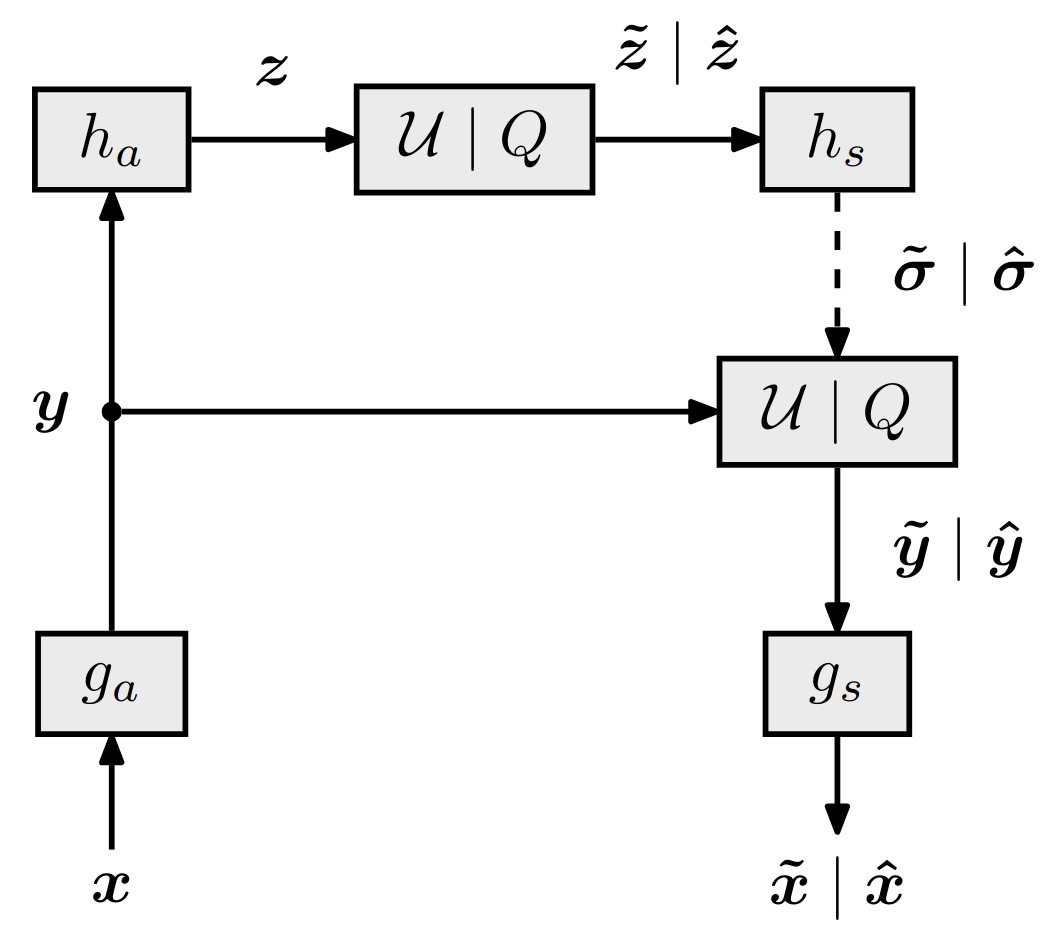
\includegraphics[width=5cm]{../img/scale_hyperprior_1.png} \label{scale_hyperprior_1:a}}
    \qquad
    \subfloat[Detailed architecture of the scale hyperprior compression model. The parameters N in the convolution layers designate the number of channels.]{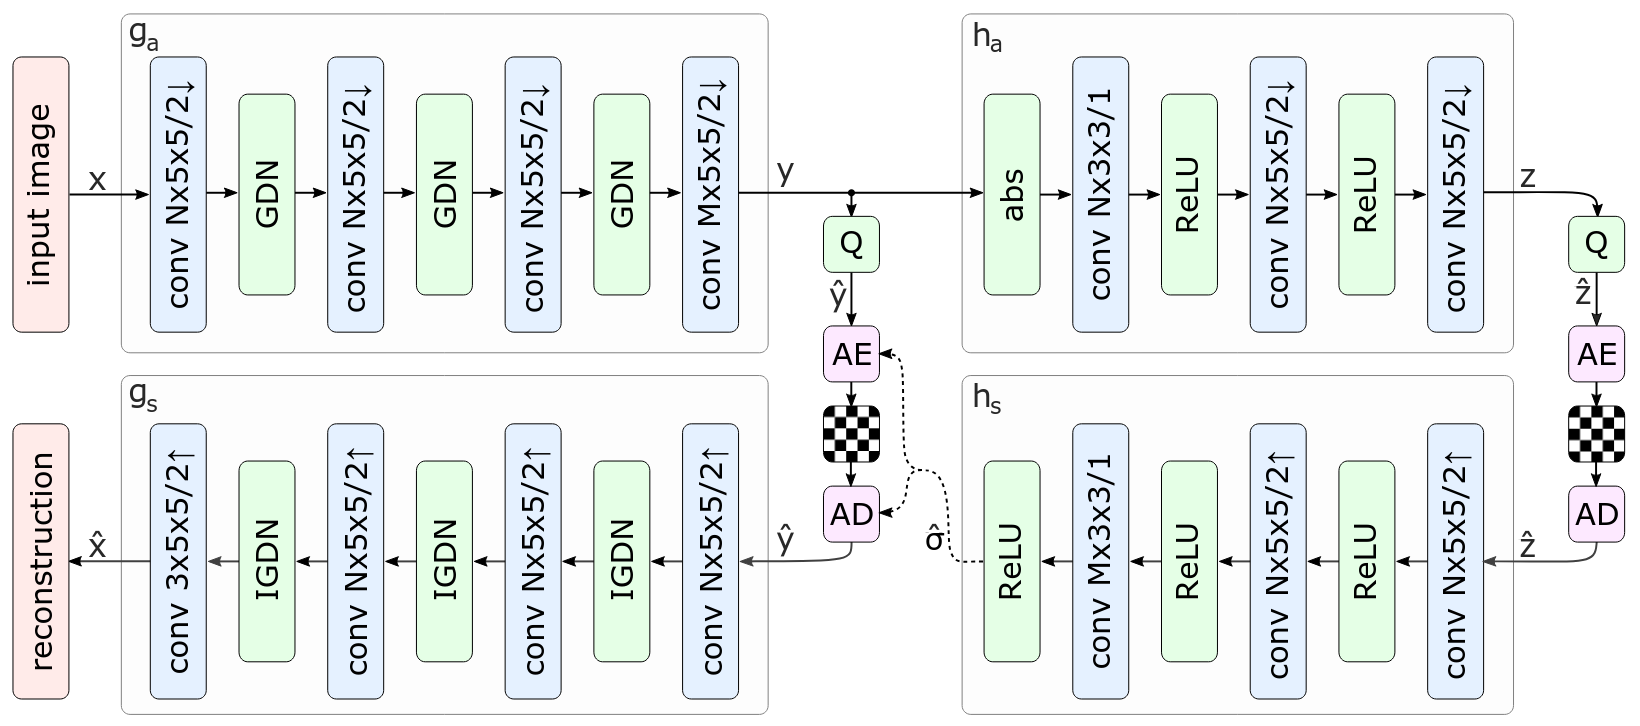
\includegraphics[width=10cm]{../img/scale_hyperprior_2.png} \label{scale_hyperprior_1:b}}
    \caption[Representations of the scale hyperprior model.]{Representations of the scale hyperprior model.}
    \label{kd_lic_2}
\end{figure}

\subsection{Training Method}
\label{training_method}
As experiments parameters are not disclosed in the scale hyperprior model paper, we use compressAI pre-trained models as our baseline comparison. For fair comparison, we match as best as we can the training method described in the compressAI documentation \cite{compressai_train}. Models were trained between 4 and 5 million steps on 256x256 image patches randomly extracted and cropped from the Vimeo90K dataset. The batch size is 16 or 32 (we choose 16). The initial learning rate is 1e-4 and decreases over time (it is divided by 2 when the evaluation loss reaches a plateau). Two different metrics can be used: \acrshort{mse} or \acrshort{msssim}. We keep the default metric (i.e. \acrshort{mse}) which corresponds to using the following loss function: \(L = \lambda\, 255^{2}\, D + R\) with \(D\) and \(R\) respectively the mean distortion and the mean estimated bit rate. The parameter \(\lambda\) allows to adjust the tradeoff between compression and image quality. Higher values give more importance to distortion encouraging the model to produce reconstructed images with high quality at the expense of bit rate. Inversely, lower values of \(\lambda\) imply more compression and more data loss. CompressAI proposes 8 pre-trained models with different values of \(\lambda\) denoted by the argument \textsf{quality}. The correspondance between this argument and the value of \(\lambda\) is summarised in Table \ref{tab_quality_lambda}. It is important to note that the \textsf{quality} argument in compressAI also impacts the network architecture (number of channels and size of the latent space). Pre-trained models with \textsf{quality} lower or equal to 5 have 128 channels and a latent space with 192 dimensions. Other pre-trained models have 192 channels and a larger latent space with 320 components. 

\begin{table}[]
    \centering
    \caption{Correspondance between the argument \textsf{quality} in compressAI and the value of \(\lambda\) when using MSE.}
    \label{tab_quality_lambda}
    \begin{tabular}{|l|c|c|c|c|c|c|c|c|}
    \hline
    \textsf{quality}             & 1 & 2 & 3 & 4 & 5 & 6 & 7 & 8 \\ \hline
    Value of \(\lambda\) for MSE & 0.0018 & 0.0035 & 0.0067 & 0.0130 & 0.0250 & 0.0483 & 0.0932 & 0.1800 \\ \hline
    \end{tabular}
\end{table}

\subsection{Testing Method}
In order to compare our results to traditional codecs or other \acrshort{lic} \acrshort{nn}, different methods can be used. In this section, we present our qualitative and quantitative testing methods.

Visual inspection is the first method that comes to mind. When dealing with lossy compression, it is necessary to assess the visual fidelity of the compressed image compared to the original image as well as other compression techniques outputs. This is done by performing meticulous visual inspection on the entire image for overall evaluation or zoomed regions of interest to analyse details.

Visual inspection is subjective and should always be crossed with quantitative measures. Several metrics can be used. Based on what is used in the litterature, we opted for the following metrics.

Image compression deals with two caracteristics: image quality and bit rate. In our study, image quality is measured with \acrshort{psnr} (and \acrfull{msssim}) and bit rate in \acrfull{bpp}. Together, they define the \acrshort{rd} performance of a compression method.

\acrshort{rd} curves are a common tool to compare compression codecs and \acrshort{nn} architectures in \acrshort{lic}. It consists in plotting the average distortion in function of the average bit rate evaluated on a set of images. Using a range of \acrshort{rd} tradeoffs allows to easily evaluate and compare the overall \acrshort{rd} performance of an architecture.

These curves can then be used to compute the Bjøntegaard Deltas for both bit rate and image quality, respectively called BD-Rate and BD-\acrshort{psnr}. As explained in \cite{barman2024bjontegaarddeltabdtutorial}, these values characterise bit rate and quality differences between two \acrshort{rd} curves (using \acrshort{psnr} as distortion metric) by measuring the area between the curves.

%#### Experiments and Results #################################################
\section{Experiments and Results}
\label{experiments_and_results}
Frugal \acrshort{ai} is an emerging concept that aims to develop models capable of "doing more with less". Frugal models consume less resources while providing great results. \acrshort{kd} is a frugal \acrshort{ai} technique that consists in using the results of a large model to help a smaller model during its training. This model's performance tends towards that of the large model. This section focuses on applying \acrshort{kd} to \acrshort{lic}. In order to do that, we first experiment with \acrshort{kd} on auto-encoders for image reconstruction. After achieving satisfactory results, we proceed in implementing \acrshort{kd} for \acrshort{lic}.

\subsection{Knowledge Distillation for Image Reconstrution}
As discussed by Ballé et al. in \cite{balle2018variationalimagecompressionscale}, \acrfull{vae} share similarities with \acrshort{lic} architectures. Both use an analysis transformation to map the input signal to a lower-dimensional latent space, followed by an approximate inverse transformation (the synthesis transform) to map the latent representation back to the signal space. However, as highlighted by Minnen et al. in \cite{minnen2018jointautoregressivehierarchicalpriors}, there is a key distinction between the two approaches. Compression is not just about reducing dimensionality; it involves reducing the entropy of the representation under a prior probability model that is shared between the sender and the receiver. Achieving high-performance image compression is, therefore, more complex than merely reconstructing images.

In this study, we explore the application of \acrshort{kd} to auto-encoders for image reconstruction, which is a more straightforward task than image compression. Initially, we familiarize ourselves with this technique by implementing it on custom-built \acrfull{ae}. Subsequently, we apply the same technique to state-of-the-art image compression models that are used as \acrshort{ae}s.

\subsubsection{Custom Auto-encoder}
This experiment investigates the application of \acrshort{kd} on well-established architectures, such as convolutional \acrshort{ae}s, and evaluates the impact of \acrshort{kd} on performance. Specifically, we train a large model (the teacher) and a smaller model (the student) both with and without \acrshort{kd}. We expect the student model, when trained with \acrshort{kd}, to achieve superior image reconstruction performance compared to the other small model. Ideally, the student model would achieve results comparable to those of the teacher model.

We design the teacher encoder with three stages each containing two convolutions with ReLU followed by a maximum pooling. This is followed by a two-layer fully connected network to achieve a latent space size of 256. The teacher decoder follows the same structure but reversed with transpose convolutions instead of convolutions and up-sampling to replace pooling. The small architecture is analogous with only one convolution (or transpose convolution) per stage. The student model is trained based on its output (by comparing the input and output images using \acrshort{mse}) but also based on the latent representation and the output of the teacher model (using \acrshort{mse} for both).

Exposed in Figure \ref{kd_ae_test_1} are the first results obtained. While mediocre in terms of \acrshort{kd} effectiveness, they highlight the importance of the "quality" of the teacher. Continuing the analogy of the teacher and student relationship, it makes sense that a good teacher is more likely to train a good student than a bad teacher. In the context of \acrshort{kd}, the student learns partially from the output of the teacher, so we must use a powerful teacher network, otherwise the student network will learn poor latent representations as well as reconstructions. In order to achieve the best possible results, we decide to perform the upcoming experiments using pre-trained networks from the compressAI model zoo as teachers. On top of dramatically reducing the training time for each experiment, it also allow us to easily compare our models to state-ot-the-art results.

\begin{figure}
    \centering
    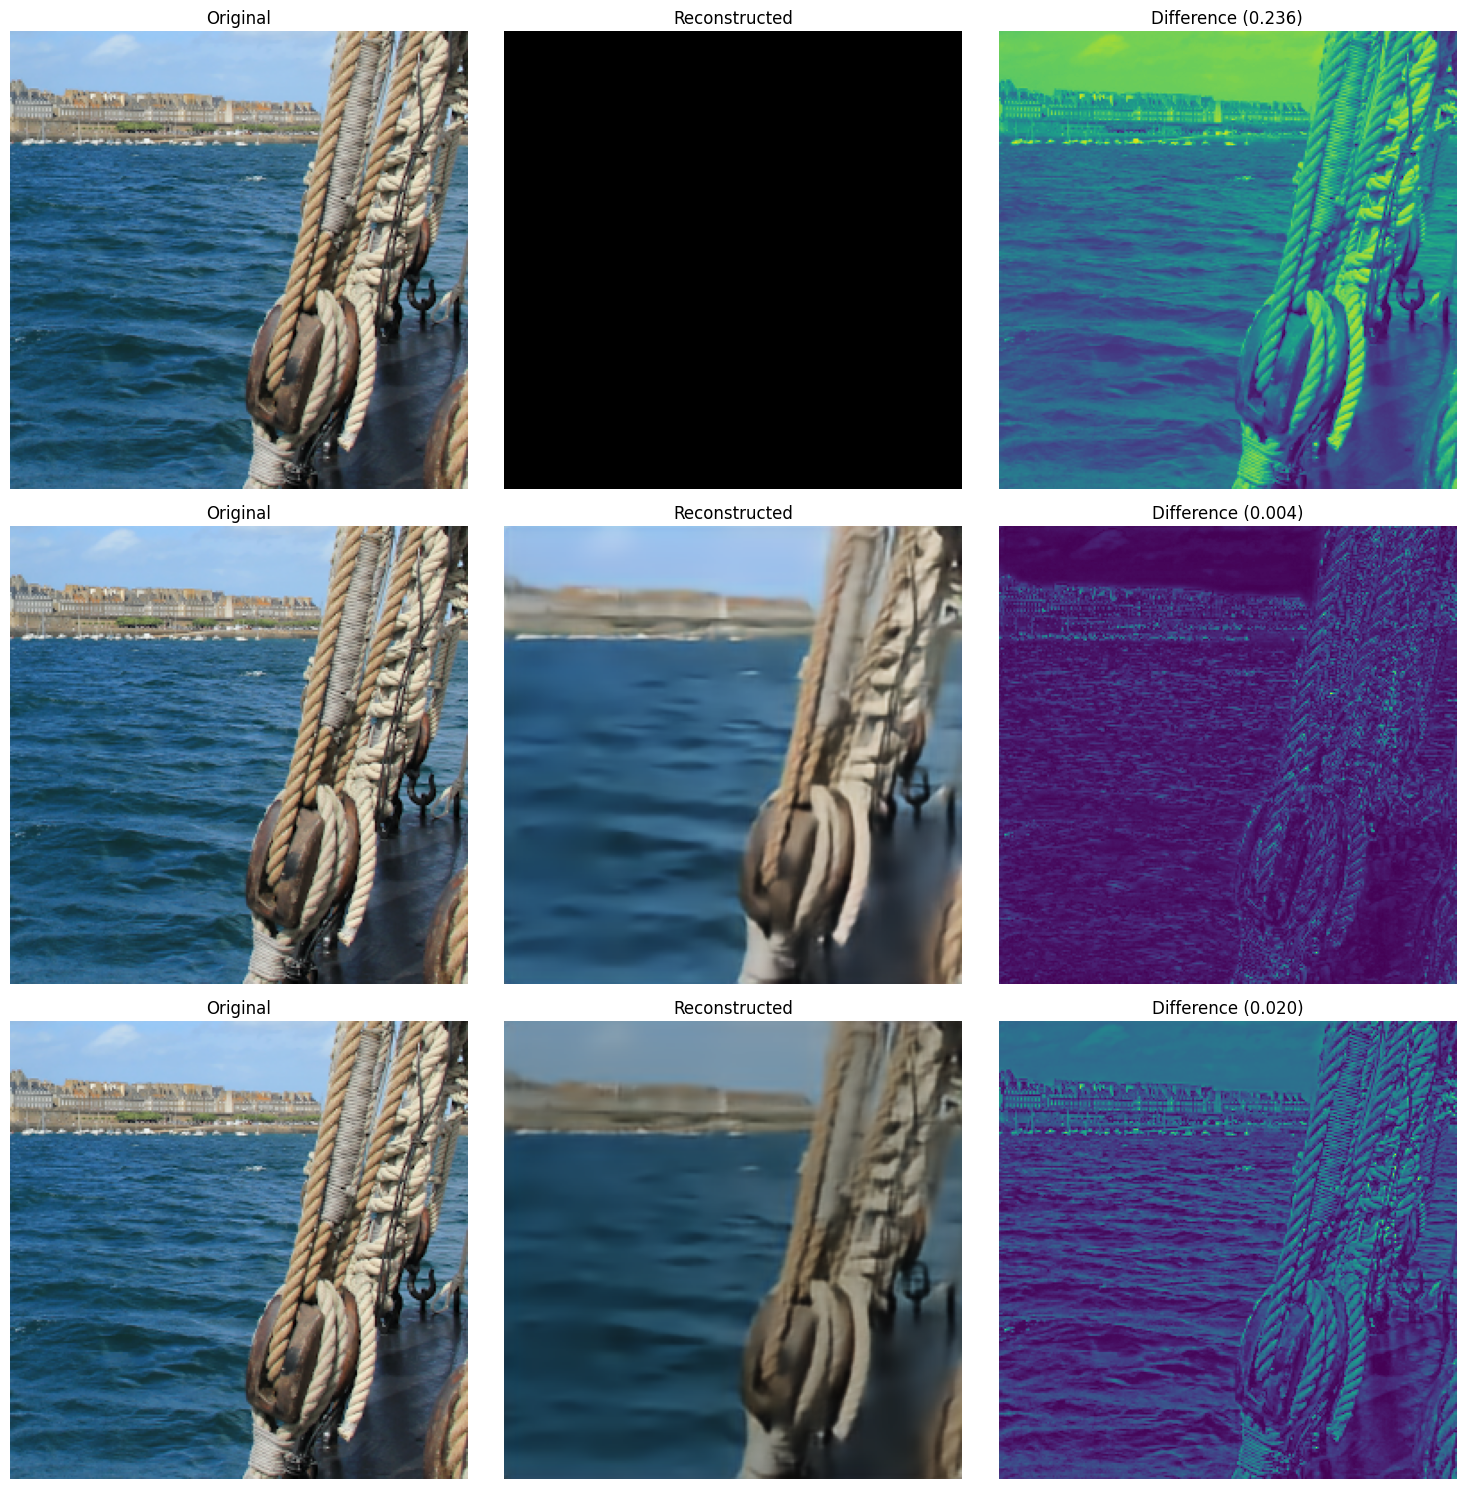
\includegraphics[width=7cm]{../img/kd_ae_test_1.png}
    \caption[Image reconstruction comparison of teacher and student architectures.]{Image reconstruction comparison of teacher and student architectures. In this experiment, the teacher (top row) converged to a degenerate solution. The student architecture without \acrshort{kd} (middle row) did not collapse and reach a \acrshort{mse} of 0.004 on this sample. When trained by the underperforming teacher, the student architecture (bottom row) suffers a performance loss: the \acrshort{mse} increases to 0.020. The impact of \acrshort{kd} is very noticable: the reconstructed image lacks details and is darker.}
    \label{kd_ae_test_1}
\end{figure}

\subsubsection{Scale Hyperprior Model as Auto-encoder}
\label{scale_hyperprior_ae}
Building on the previous section, which highlighted the benefits of \acrshort{kd} for auto-encoders, we now turn our attention to applying this technique to image compression. With this in mind, we take a step-by-step approach, beginning with an attempt to observe similar results using architectures designed for image compression. The objective of the following experiment is to employ the state-of-the-art scale hyperprior model as an \acrshort{ae} for image reconstruction. As mentioned earlier, image reconstruction closely resembles image compression, but without the entropy constraint on the latent space. Since the scale hyperprior model is designed for \acrshort{lic}, we expect it to perform well on this less challenging task.\footnote{An additional benefit of this experiment is that it provides a code foundation for following experiments focused on \acrshort{lic}.}

The following experiment consists in training five students models with different architectures. Using the pre-trained scale hyperprior model optimised for \acrshort{mse} with \textsf{quality} set to 5 (with 128 channels and a latent space of size 192) as teacher, we train models with different number of channels. We define five models with 16, 32, 64, 96 and 112 channels while preserving the size of the latent space. We use the following \acrshort{kd} loss function:

\begin{equation}
    L = \lambda_{1}\, MSE(\hat{y}_{student}, \hat{y}_{teacher}) + \lambda_{2}\, MSE(\hat{x}_{student}, \hat{x}_{teacher}) + \lambda_{3}\, MSE(\hat{x}_{student}, x)
    \label{loss_1}
\end{equation}

We use the following set of parameters: \(\{\lambda_{1}, \lambda_{2}, \lambda_{3}\} = \{0.2, 0.2, 0.6\}\) and train the models with the method defined in Section \ref{training_method}: 1000 epochs on the Vimeo90K dataset with a base learning rate of \(10^{-4}\).

Figure \ref{kd_ae_1:a} shows reconstructions of image 14 of the Kodak dataset with the teacher and all student networks. As axpected, the teacher (a pre-trained model) propose a reconstructed image virtually undistinguishable from the orignal one. As for the students, eventhough they give visually satisfying results, the models with less parameters do not retain as much details. The reconstructed image appears a little bit blurry. As expected, the more the student architecture is similar to the teacher (that is to say, more channels), the more it is able to reach the same performance as the teacher. This is quantitatively measured using MSE on Figure \ref{kd_ae_1:b}.

\begin{figure}[H]
    \centering
    \subfloat[Reconstruction results on image 14 of the Kodak dataset with teacher and student architectures.]{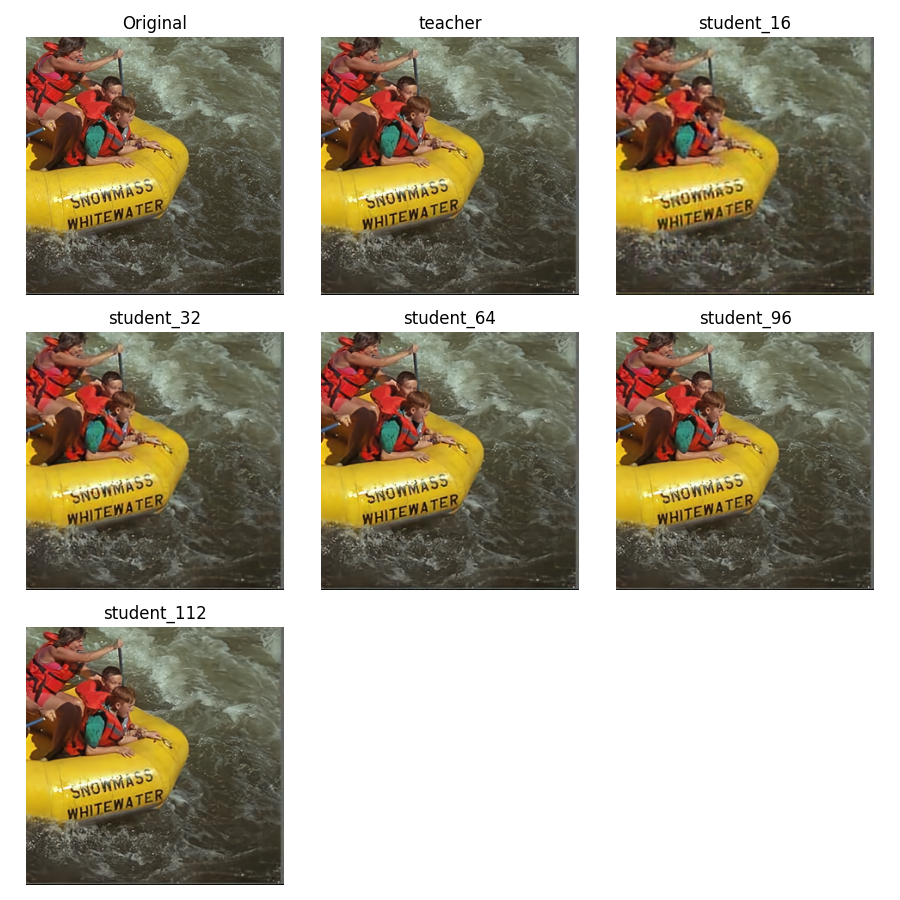
\includegraphics[width=7cm]{../img/kd_ae_kodak_14.png} \label{kd_ae_1:a}}
    \qquad
    \subfloat[Average \acrshort{mse} curve on the Kodak dataset for students with different number of channels.]{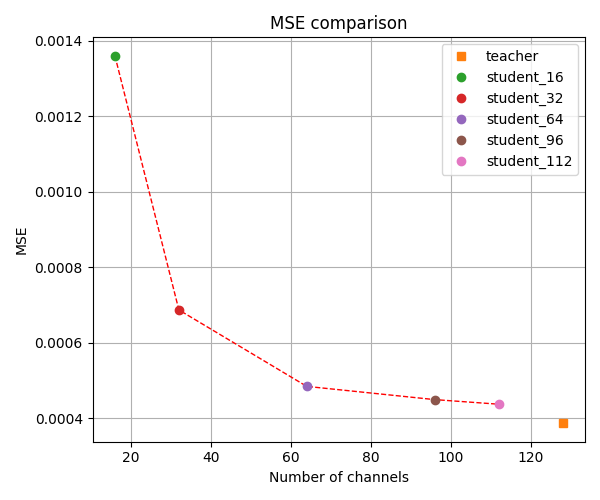
\includegraphics[width=7cm]{../img/kd_ae_mse.png} \label{kd_ae_1:b}}
    \caption[Evaluation on the Kodak dataset of the scale hyperprior student models trained for image reconstruction.]{Evaluation on the Kodak dataset of the scale hyperprior student models trained for image reconstruction. Student models with fewer channels propose less detailed image reconstruction. This is noticeable on single image reconstructions or on average using \acrshort{mse} measures.}
    \label{kd_ae_1}
\end{figure}

For reference, we show in Figure \ref{kd_ae_2} the \acrshort{rd} performance of the student models. It should be noted that the teacher network used in this experiment was trained for image compression tasks so one could argue that these models are not exactly auto-encoders for image reconstruction. What is sure is that they are far from state-of-the-art models in image compression tasks. What remains to be seen is to what extent a properly defined \acrshort{kd} loss for \acrshort{lic} does increase the \acrshort{rd} performance of these student models. This, as well as discussion related to the benefits of smaller student models for \acrshort{lic}, is the subject of the next section.

\begin{figure}
    \centering
    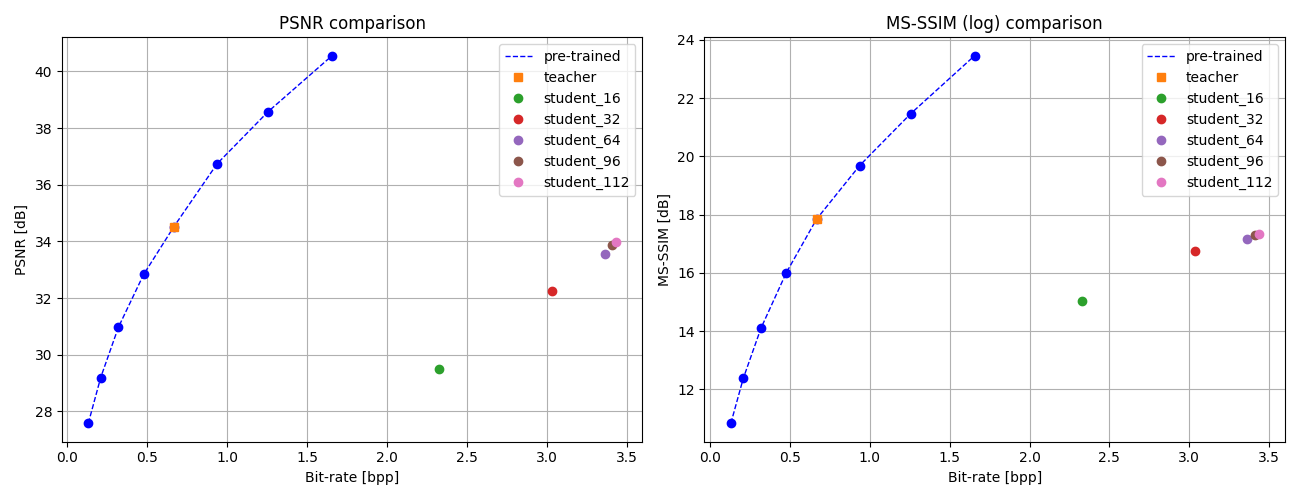
\includegraphics[width=15cm]{../img/kd_ae_rd.png}
    \caption[Average \acrshort{rd} performance on the Kodak dataset for students with different number of channels.]{Average \acrshort{rd} performance on the Kodak dataset for students with different number of channels. Eventhough they were guided by a \acrshort{lic} model during their training, the student models poorly compares to state-of-the-art models in \acrshort{rd}. (The pre-trained models are compressAI scale hyperperior models with \extsf{quality} from 1 to 8).}
    \label{kd_ae_2}
\end{figure}

Whether it is for custom convolutional \acrshort{ae} or models specifically designed for \acrshort{lic}, there is no denial that \acrshort{kd} positively influence the performance of small models. This section certify this result for image reconstruction, we now transfer this technique to \acrshort{lic} domain.

\subsection{Knowledge Distillation for Image Compression}
Having assessed the effectiveness of \acrshort{kd} for computer vision tasks similar to image compression, we investigate the success of this frugal \acrshort{ai} technique on \acrshort{nn}-based image compression. Still using the scale hyperprior model introduced in \cite{balle2018variationalimagecompressionscale}, we train a serie of student models with \acrshort{kd} to evaluate both their \acrshort{rd} performance and their ability to be deployed on resource constrained platforms.

\subsubsection{Rate-Distortion Performance}
This section aims at evaluating the \acrshort{rd} performance gain achievable through \acrshort{kd}. By guiding small models during their training with a teacher model, we hope to increase their ability to compress images. We first explain our method then we present our results.

\paragraph{Method}
\acrshort{lic} distinguish itself from other computer vision tasks (such as dimensionality reduction) by minimising the entropy of the latent representation. In dimensionality reduction, the latent representation has no practical application. When it comes to image compression, it is the latent representation of the image that will be stored or transmitted. Having the smallest possible entropy allows for a smaller entropy coding which means less bits to handle in real world applications. This is why the rate-distortion loss is used in \acrshort{lic} as it allows to find a tradeoff between image quality and bit rate according that fits the requirements of the application. In order to have similar results with \acrshort{lic}, the previous loss function, introduced in Equation \eqref{loss_1}, is updated as follow:

\begin{align}
    L = \lambda_{1}\, MSE(\hat{y}_{student}, \hat{y}_{teacher}) + \lambda_{2}\, MSE(\hat{x}_{student}, \hat{x}_{teacher}) + \lambda_{3}\, RD(\hat{y}_{student}, \hat{x}_{student}, x)\label{loss_2}\\
    RD(\hat{y}_{student}, \hat{x}_{student}, x) = -E[\log_{2}\hat{y}_{student} + \log_{2}\hat{z}_{student}] + \lambda\, MSE(\hat{x}_{student}, x)
\end{align}

We also tried to use the Kullback-Leibler divergence instead of \acrshort{mse} loss function on the latent space but found that it resulted in slightly higher bit rates. Outcome of this experiment is exposed in Figure \ref{appendix:kd_lic_1_kld}.

For easier comparison and because our study focuses on low bit rate image compression, we compare our results to compressAI pre-trained models with \textsf{quality} from 1 to 5.

\paragraph{Architecture Size Tradeoff}
\label{architecture_size_tradeoff}
The objective of \acrshort{kd} is to improve the performance of small models using a large one. However, there is no definition of "a small model" so we start by experimenting with model sizes. Following our training method, we create five new models using \acrshort{kd} and the loss function from Equation \ref{loss_2}. We use \(\lambda = 0.025\) in the \acrshort{rd} part of the loss, the same value used by the teacher model during its training. The five models have different sizes. We modify their architecture by changing the number of channels. The smallest deals with as few as 16 channels while the largest student has 112 (number of channels is indicated by the parameter N in Figure \ref{scale_hyperprior_1:b}). It should be noted that the size of the latent space remains the same across all models, teacher and students.

Unsurprisingly, using \acrshort{RD} loss yields far better results for image compression. Contrary to similar models trained with \acrshort{mse} only (Section \ref{scale_hyperprior_ae}), these new models can be found in the same operational \acrshort{rd} area as state-of-the-art models (Figure \ref{kd_lic_1}).

Results depicted in Figure \ref{kd_lic_1} follow our intuition. Students with larger number of channels (i.e. 64, 96 and 112) take full advantage of \acrshort{kd} and reach roughly the same \acrshort{bpp} and \acrshort{psnr} as the teacher. Models with 16 and 32 channels cannot reach the same level of image quality. Both of them end up far behind pre-trained models in \acrshort{rd} performance and results in higher \acrshort{mse} error (Figure \ref{kd_lic_2:b}). Eventhough they produce visually impressive results (Figure \ref{kd_lic_2:a}) for models with so few parameters, they are not relevant candidates when taking into account only \acrshort{rd} performance. The number of channels definitely impact the output quality in extreme scenarios (e.g. very few channels) but can be reduced to some extend without degrading image quality.

\begin{figure}
    \centering
    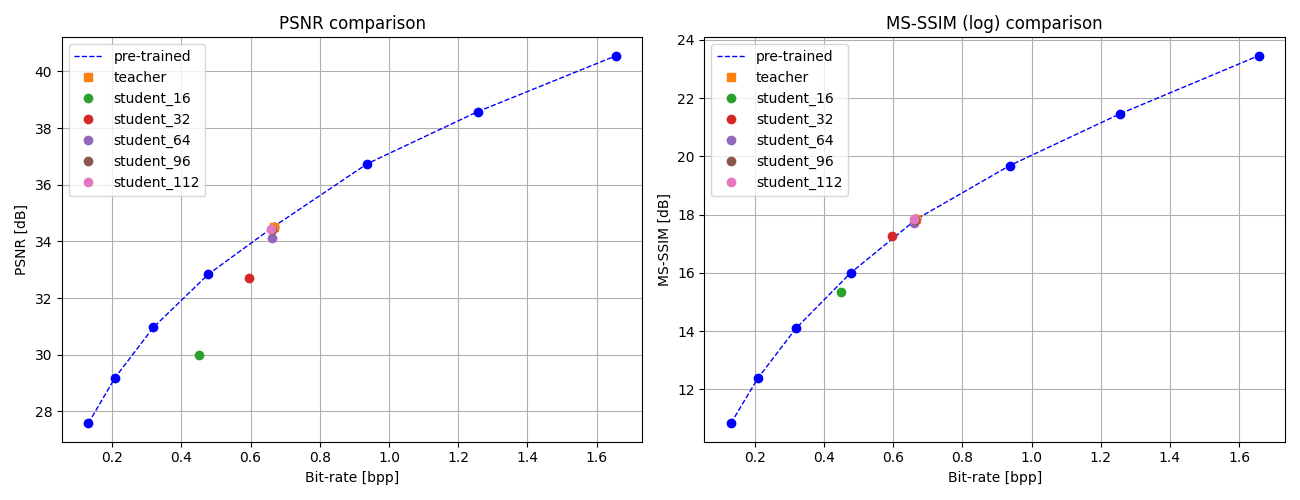
\includegraphics[width=15cm]{../img/kd_lic_rd_channels.png}
    \caption[Average \acrshort{rd} curve on the Kodak dataset for students with different number of channels.]{Average \acrshort{rd} curve on the Kodak dataset for students with different number of channels. Despite being trained similarly, all models have different outputs. Models with at least 64 channels performs alike their teacher but 16 and 32 channels are not sufficient to preserve the same image quality.}
    \label{kd_lic_1}
\end{figure}
% Use 263674, 274457, 274461, 274464, 263691

\begin{figure}[H]
    \centering
    \subfloat[Reconstruction results on image 14 of the Kodak dataset with teacher and student architectures.]{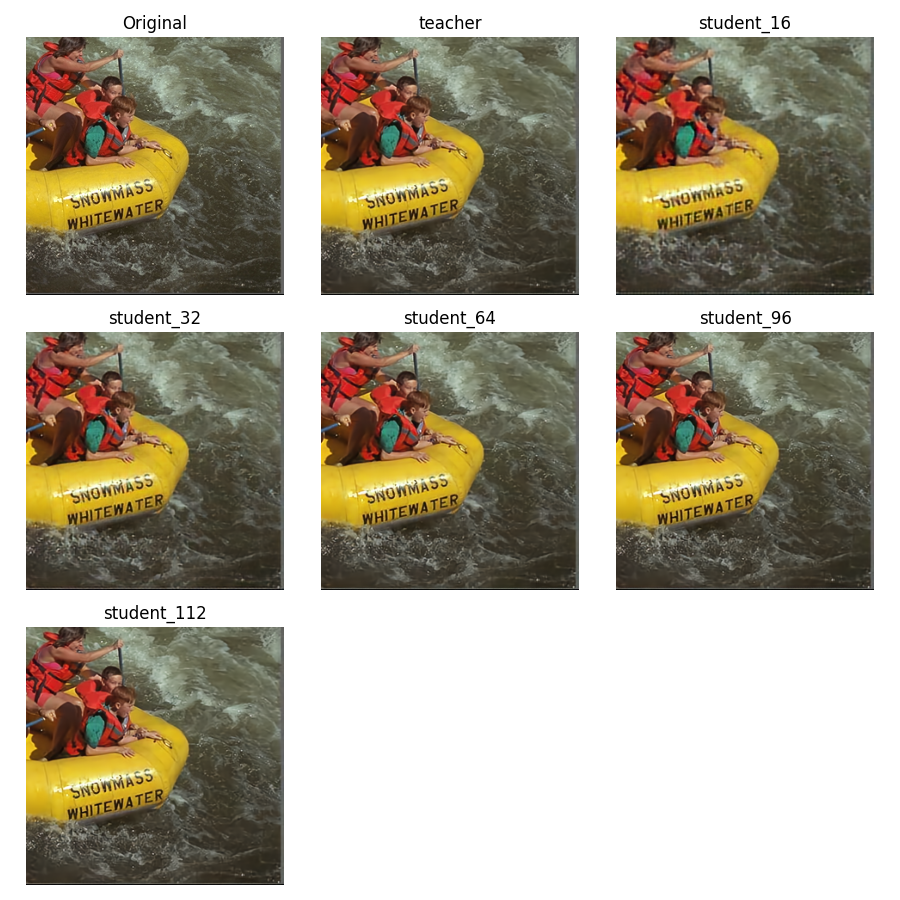
\includegraphics[width=7cm]{../img/kd_lic_kodak_14.png} \label{kd_lic_2:a}}
    \qquad
    \subfloat[Average MSE curve on the Kodak dataset for students with different number of channels.]{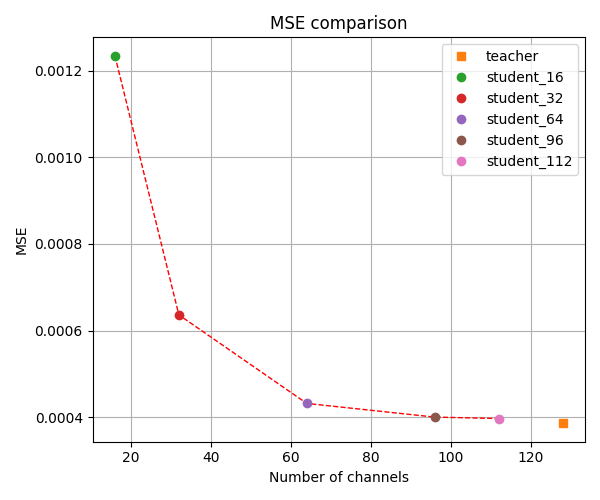
\includegraphics[width=7cm]{../img/kd_lic_mse.png} \label{kd_lic_2:b}}
    \caption[Evaluation on the Kodak dataset of the scale hyperprior student models trained for image compression.]{Evaluation on the Kodak dataset of the scale hyperprior student models trained for image compression. Meticulous visual inspection and average \acrshort{mse} of the output prove the importance of the number of channels when limiting compression loss.}
    \label{kd_lic_2}
\end{figure}

\paragraph{Rate-Distortion Tradeoff}
Once again, following our training method, we train five new models using \acrshort{kd} and the loss function from Equation \ref{loss_2}. The teacher model is still taken from the compressAI zoo with \textsf{quality} set to 5. This time, we fix the number of channels across all models (i.e. 64, the smallest number of channels that did not degrade too much performance in previous experiments) but we use different values of \(\lambda\) in the \acrshort{rd} part of the loss. For easier comparison and because our study focuses on low bit rate image compression, we use the values of \(\lambda\) corresponding to the five lowest values of \textsf{quality} (Table \ref{tab_quality_lambda}). We use the pre-trained models corresponding to the same values of \(\lambda\) as a baseline to compare our results.

As a reminder, the pre-trained models in Figure \ref{kd_lic_4} all have 128 channels. This means that our student models all have half as many channels as the pre-trained models do. Still, all students have similar or higher \acrshort{psnr} than their pre-trained counter-part. More precisely, when quality is prioritised (student 4 and 5), \acrshort{kd} is not the ideal solution: the models performs better than what they would have if trained alone but they are restrained by the modest number of channels. Student 5 attain the limit of what is feasible with 64 channels: with the same \acrshort{rd} tradeoff as the teacher, it is not able to match the teacher image quality. However, smaller models (student 1, 2 and 3) trained to prioritise bit rate reach better \acrshort{psnr} thanks to the teacher model (trained to favorise image quality) pulling them toward the top of the chart. Another interesting experiment is to use a teacher trained to prioritize bit rate. In that case, we observe that all students are pushed toward the bottom left of the chart (Figure \ref{kd_lic_4_bis}). This compromise could be useful for storage or bandwidth critical operations.

\begin{figure}
    \centering
    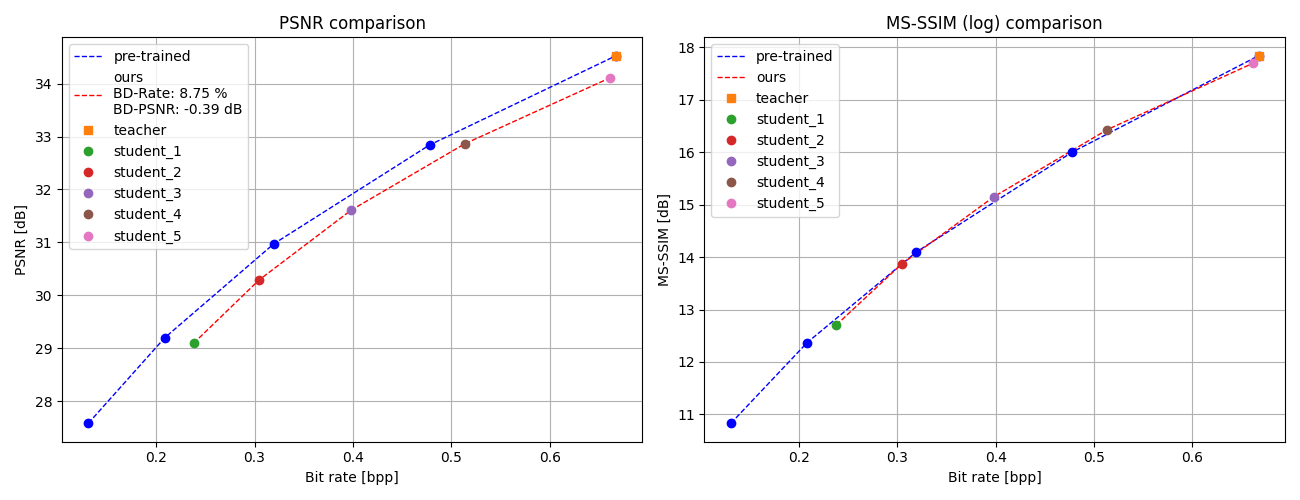
\includegraphics[width=15cm]{../img/kd_lic_rd_lambda_1.png}
    \caption[Average \acrshort{rd} curve on the Kodak dataset for students with different \acrshort{rd} tradeoffs.]{Average \acrshort{rd} curve on the Kodak dataset for students with different \acrshort{rd} tradeoffs. Trained by a teacher with an emphasis on image quality, students 1, 2 and 3 achieve better \acrshort{psnr} than their pre-trained counterpart. Students 4 and 5 are held back by the limited number of channels.}
    \label{kd_lic_4}
\end{figure}
% Use 280392, 281662, 281976, 281979, 274461

\begin{figure}
    \centering
    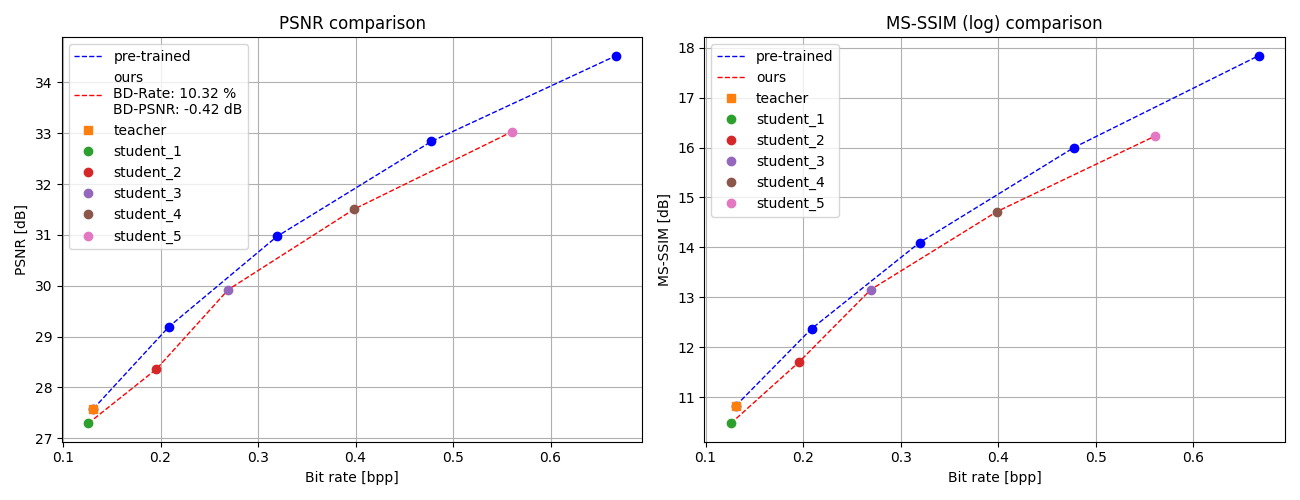
\includegraphics[width=15cm]{../img/kd_lic_rd_lambda_2.png}
    \caption[Average \acrshort{rd} curve on the Kodak dataset for students with different \acrshort{rd} tradeoffs and a teacher focusing on minimising bit rate.]{Average \acrshort{rd} curve on the Kodak dataset for students with different \acrshort{rd} tradeoffs and a teacher focusing on minimising bit rate. Student \acrshort{nn}s, influenced by they teacher at training time, have a lower bit rate than their pre-trained counterpart. The gap becomes more noticeable as \(lambda\) increases. This gain in bit rate implies a loss in image quality across all students.}
    \label{kd_lic_4_bis}
\end{figure}
% Use 289751, 295889, 289745, 296544, 289742

This section proves that \acrshort{kd} can be successfully applied to \acrshort{lic} tasks. We are able to train small models with \acrshort{rd} performance almost on par with larger models. But \acrshort{rd} performance is only one part of the equation with frugal \acrshort{ai}: we now need to assess the resource savings. It remains to be seen if it is worth making the tradeoff of loosing some \acrshort{rd} performance to use smaller models.

\subsubsection{Application to Resource Constrained Platfroms}
\label{application_resource_contrained_platforms}
Real life applications for \acrshort{lic} do not only focus on \acrshort{rd} performance. It is important to ensure great image quality at the lowest bit rate possible but other parameters need to be taken into account. Having proved the effectiveness of \acrshort{kd} for \acrshort{lic} tasks in terms of \acrshort{rd} performance with small student models almost on par with larger models, we now need to put into perspective these results. Let us dive into the second apsect of this study: making \acrshort{lic} possible on resource-limited platforms. This section analyses student models with different architectures from a resource stand point across three main axis: memory, computing power and energy consumption.

In this section, we use the models first introduced in Section \ref{architecture_size_tradeoff}. There are five student architectures with 16, 32, 64, 96 and 112 channels and a latent space of size 192. We compare our models to pre-trained models from the compressAI zoo (with \textsf{quality} ranging from 1 to 5).

Most resource constrained computers deal with a limited amount of memory. This limiting factor sometimes makes them unsuitable for tasks requiring large models. In \acrshort{lic}, distillation allows to use smaller models without degrading \acrshort{rd} performance. Our student models can have as few as 0.27 M parameters while standard models have 5 M parameters. This is a reduction of up to 95 \% in terms of parameters or memory size. Values for each student model are presented in Table \ref{tab_size}. While the number of parameters definitely impact \acrshort{rd} capabilities of \acrshort{nn}, Figures \ref{kd_lic_parameters} and \ref{appendix:kd_lic_memory} show that student models with 64 channels and above are quite close to their teacher in both \acrshort{psnr} and bit rate. In other words, these model could be used instead of the teacher on devices with limited memory without noticeably degrading the user experience. The student with 64 channels is particularly valuable as it offers \acrshort{psnr} and bit rate inline with the teacher while reducing the memory footprint by 68 \%.

\begin{figure}
    \centering
    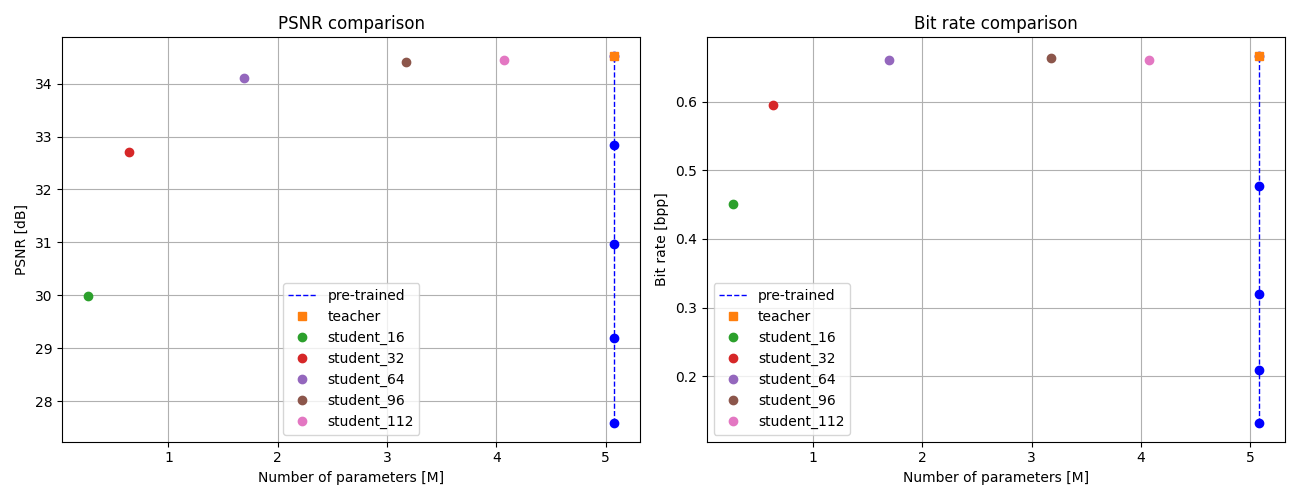
\includegraphics[width=15cm]{../img/kd_lic_parameters.png}
    \caption[\acrshort{psnr} and bit rate on the Kodak dataset according to students number of parameters.]{\acrshort{psnr} and bit rate on the Kodak dataset according to students number of parameters. Reducing the number of parameters graduatly decrease \acrshort{rd} results. Similar results are observed for memory footprint. In our testing, a fair balance between \acrshort{rd} and memory footprint is using 64 channels as it virtually does not degrade performance while reducing the memory footprint by 68 \%.}
    \label{kd_lic_parameters}
\end{figure}

\begin{table}[]
    \centering
    \caption[Number of parameters, memory footprint, \acrshort{psnr} and bit rate for teacher and student models.]{Number of parameters, memory footprint, \acrshort{psnr} and bit rate for teacher and student models.}
    \label{tab_size}
    \begin{tabular}{|c|c|lr|lr|lr|lr|}
        \hline
        Model                    & \begin{tabular}[c]{@{}c@{}}Number\\ of channels\end{tabular} & \multicolumn{2}{c|}{\begin{tabular}[c]{@{}c@{}}Number of\\ parameters {[}M{]}\end{tabular}} & \multicolumn{2}{c|}{\begin{tabular}[c]{@{}c@{}}Memory\\ footprint {[}MB{]}\end{tabular}} & \multicolumn{2}{c|}{PSNR} & \multicolumn{2}{c|}{\begin{tabular}[c]{@{}c@{}}Bit rate\\ {[}bpp{]}\end{tabular}} \\ \hline
        Teacher                  & 128                                                          & {\color[HTML]{656565} }                          & 5.08                                     & {\color[HTML]{656565} }                        & 20.18 & {\color[HTML]{656565} }          & 34.53 & {\color[HTML]{656565} }          & 0.67 \\ \hline
        \multirow{5}{*}{Student} & 112                                                          & {\color[HTML]{656565} -19.77 \%}                 & 4.07                                     & {\color[HTML]{656565} -23.03 \%}               & 15.53 & {\color[HTML]{656565} -0.26 \%}  & 34.44 & {\color[HTML]{656565} -1.03 \%}  & 0.66 \\ \cline{2-10} 
                                 & 96                                                           & {\color[HTML]{656565} -37.47 \%}                 & 3.17                                     & {\color[HTML]{656565} -40.01 \%}               & 12.11 & {\color[HTML]{656565} -0.33 \%}  & 34.41 & {\color[HTML]{656565} -0.58 \%}  & 0.66 \\ \cline{2-10} 
                                 & 64                                                           & {\color[HTML]{656565} -66.62 \%}                 & 1.69                                     & {\color[HTML]{656565} -67.98 \%}               & 6.46  & {\color[HTML]{656565} -1.21 \%}  & 34.11 & {\color[HTML]{656565} -0.91 \%}  & 0.66 \\ \cline{2-10}
                                 & 32                                                           & {\color[HTML]{656565} -87.46 \%}                 & 0.64                                     & {\color[HTML]{656565} -87.97 \%}               & 2.43  & {\color[HTML]{656565} -5.25 \%}  & 32.71 & {\color[HTML]{656565} -10.73 \%} & 0.60 \\ \cline{2-10} 
                                 & 16                                                           & {\color[HTML]{656565} -94.77 \%}                 & 0.27                                     & {\color[HTML]{656565} -94.98 \%}               & 1.01  & {\color[HTML]{656565} -13.17 \%} & 29.98 & {\color[HTML]{656565} -32.44 \%} & 0.45 \\ \hline
    \end{tabular}
\end{table}

Computers can only perform a certain amount of operations per unit of time. When using with mainstream hardware, the computing power required to use an image compression model like the scale hyperprior model is sufficient. However, when dealing with resource constrained devices, the latency might increase which goes against the objective of real-time decompression. With too much latency, it is impossible too extend image decompression to video decompression. Here, we focus on two metrics: the number of \acrfull{flop}s (i.e. the number of floating-point operations carried out to run an inference) and the model throughput (i.e. the number of frames that can process the model in one second). According to our results, the student with 16 channels only requires 3 \% of the teacher \acrshort{flop}s to perform the inference which translates to a 25 \% increase in throughput (Table \ref{tab_compute}). Figures \ref{kd_lic_flop} and \ref{kd_lic_fps} show that once again, the student with 64 channels represents the best compromise between \acrshort{rd} and \acrshort{flop}s or throughput. It should also be noted that all our models present a throughput that exceeds all requirements for video streaming. This headroom can be used in different ways: we can either increase the stream resolution to enhance user experience or reduce the inference frequency to save energy. 

\begin{figure}
    \centering
    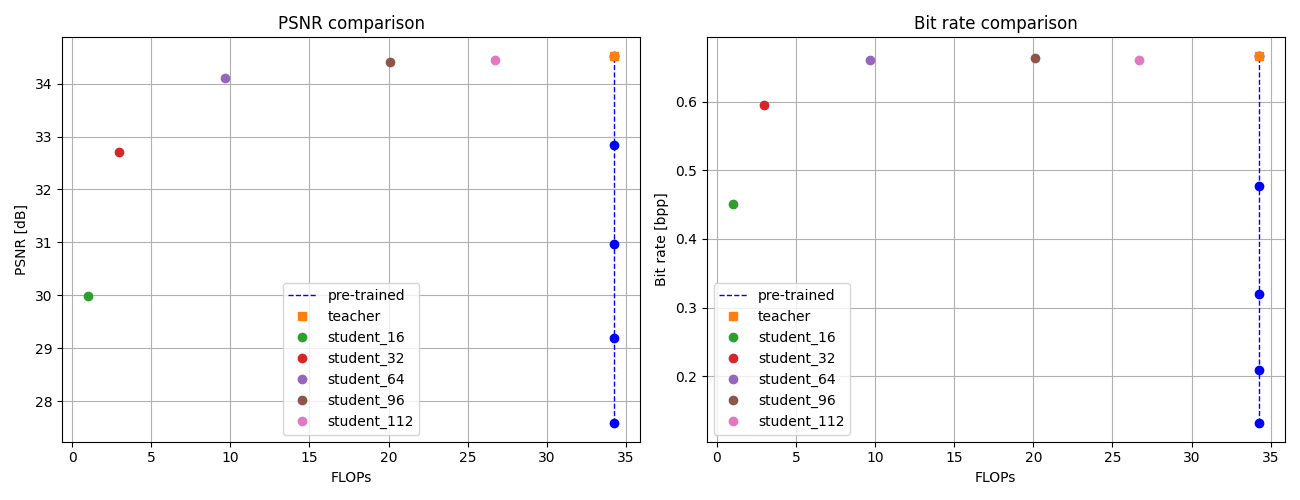
\includegraphics[width=15cm]{../img/kd_lic_flop.png}
    \caption[\acrshort{psnr} and bit rate on the Kodak dataset according to students \acrshort{flop}s.]{\acrshort{psnr} and bit rate on the Kodak dataset according to students \acrshort{flop}s. Our knowledge distilled models are good candidates for devices with limited compute power. They all offer lower \acrshort{flop} counts than standard models. However, this comes at a non-negligeable cost in image quality and bit rate for the smallest models.}
    \label{kd_lic_flop}
\end{figure}

\begin{figure}
    \centering
    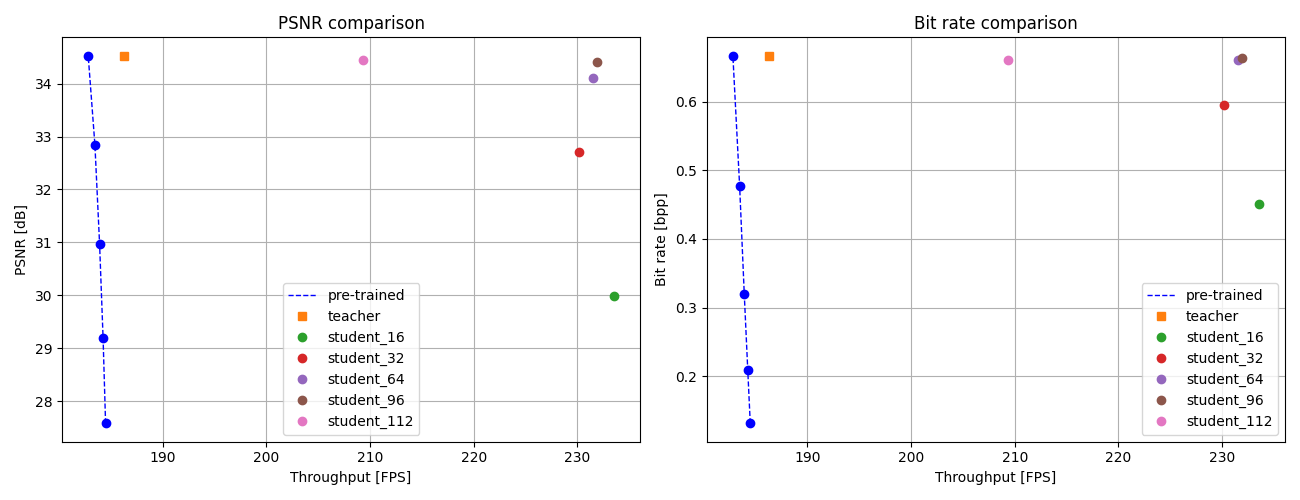
\includegraphics[width=15cm]{../img/kd_lic_fps.png}
    \caption[\acrshort{psnr} and bit rate on the Kodak dataset according to students throughput.]{\acrshort{psnr} and bit rate on the Kodak dataset according to students throughput. All models, exceed standard frame rate. With, higher throughput than pre-trained models, our knowledge distilled models have more headroom for higher resolution frames or lower energy consumption depending the real world application.}
    \label{kd_lic_fps}
\end{figure}

\begin{table}[]
    \centering
    \caption[\acrshort{flop}s, throughput, \acrshort{psnr} and bit rate for teacher and student models.]{\acrshort{flop}s, throughput, \acrshort{psnr} and bit rate for teacher and student models.}
    \label{tab_compute}
    \begin{tabular}{|c|c|lr|lr|lr|lr|}
    \hline
    Model                    & \begin{tabular}[c]{@{}c@{}}Number\\ of channels\end{tabular} & \multicolumn{2}{c|}{\begin{tabular}[c]{@{}c@{}}Floating point\\ operations\\ {[}GFLOP/frame{]}\end{tabular}} & \multicolumn{2}{c|}{\begin{tabular}[c]{@{}c@{}}Throughput\\ {[}FPS{]}\end{tabular}} & \multicolumn{2}{c|}{PSNR} & \multicolumn{2}{c|}{\begin{tabular}[c]{@{}c@{}}Bit rate\\ {[}bpp{]}\end{tabular}} \\ \hline
    Teacher                  & 128                                                          & {\color[HTML]{656565} }                                & 34.24                                             & {\color[HTML]{656565} }                     & 184.20 & {\color[HTML]{656565} }          & 34.53 & {\color[HTML]{656565} }          & 0.67 \\ \hline
    \multirow{5}{*}{Student} & 112                                                          & {\color[HTML]{656565} -22.01 \%}                       & 26.70                                             & {\color[HTML]{656565} +13.47 \%}            & 209.01 & {\color[HTML]{656565} -0.26 \%}  & 34.44 & {\color[HTML]{656565} -1.03 \%}  & 0.66 \\ \cline{2-10} 
                             & 96                                                           & {\color[HTML]{656565} -41.31 \%}                       & 20.10                                             & {\color[HTML]{656565} +25.74 \%}            & 231.61 & {\color[HTML]{656565} -0.33 \%}  & 34.41 & {\color[HTML]{656565} -0.58 \%}  & 0.66 \\ \cline{2-10}
                             & 64                                                           & {\color[HTML]{656565} -71.75 \%}                       & 9.67                                              & {\color[HTML]{656565} +26.20 \%}            & 232.47 & {\color[HTML]{656565} -1.21 \%}  & 34.11 & {\color[HTML]{656565} -0.91 \%}  & 0.66 \\ \cline{2-10} 
                             & 32                                                           & {\color[HTML]{656565} -91.31 \%}                       & 2.98                                              & {\color[HTML]{656565} +25.89 \%}            & 231.90 & {\color[HTML]{656565} -5.25 \%}  & 32.71 & {\color[HTML]{656565} -10.73 \%} & 0.60 \\ \cline{2-10}
                             & 16                                                           & {\color[HTML]{656565} -97.01 \%}                       & 1.02                                              & {\color[HTML]{656565} +26.83 \%}            & 233.63 & {\color[HTML]{656565} -13.17 \%} & 29.98 & {\color[HTML]{656565} -32.44 \%} & 0.45 \\ \hline
    \end{tabular}
\end{table}

Most edge devices also have access to a limited amount of energy whether it is in time because they run on battery like smartphones or because they are \acrfull{iot} devices that run 24/7 and thus should not consume a lot of energy. This is why we focus on the energy required to process a single frame. Table \ref{tab_energy} shows that we can save up to 60 \% of the energy used by the teacher model by using the student with 16 channels. Using Figure \ref{kd_lic_energy}, that the model that offers the best tradeoff between \acrshort{psnr} and energy consumption in the student model with 64 channels. By using this model we keep the same image quality while reducing our energy consumption by 35 \%.

\begin{figure}
    \centering
    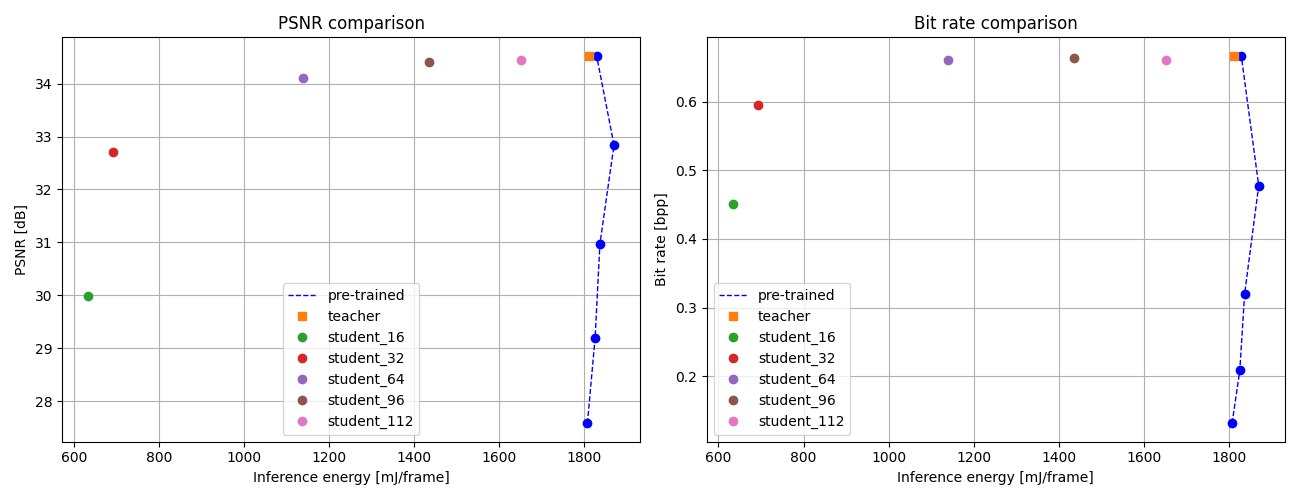
\includegraphics[width=15cm]{../img/kd_lic_energy.png}
    \caption[\acrshort{psnr} and bit rate on the Kodak dataset according to students consumed energy.]{\acrshort{psnr} and bit rate on the Kodak dataset according to students consumed energy. \acrshort{kd} is a great method to create energy friendly \acrshort{lic} models. If energy consumption is not too restricted, we recommand using the student with 64 channels that consumes 35 \% less energy per frame and achieve image compression on par with the teacher model.}
    \label{kd_lic_energy}
\end{figure}

\begin{table}[]
    \centering
    \caption[Consumed energy, \acrshort{psnr} and bit rate for teacher and student models.]{Consumed energy, \acrshort{psnr} and bit rate for teacher and student models.}
    \label{tab_energy}
    \begin{tabular}{|c|c|lr|lr|lr|}
        \hline
        Model                    & \begin{tabular}[c]{@{}c@{}}Number\\ of channels\end{tabular} & \multicolumn{2}{c|}{\begin{tabular}[c]{@{}c@{}}Energy\\ {[}mJ/frame{]}\end{tabular}} & \multicolumn{2}{c|}{PSNR} & \multicolumn{2}{c|}{\begin{tabular}[c]{@{}c@{}}Bit rate\\ {[}bpp{]}\end{tabular}} \\ \hline
        Teacher                  & 128                                                          & {\color[HTML]{656565} }                     & 1767.85 & {\color[HTML]{656565} }          & 34.53 & {\color[HTML]{656565} }          & 0.67 \\ \hline
        \multirow{5}{*}{Student} & 112                                                          & {\color[HTML]{656565} -9.47 \%}             & 1600.41 & {\color[HTML]{656565} -0.26 \%}  & 34.44 & {\color[HTML]{656565} -1.03 \%}  & 0.66 \\ \cline{2-8} 
                                 & 96                                                           & {\color[HTML]{656565} -19.88 \%}            & 1416.34 & {\color[HTML]{656565} -0.33 \%}  & 34.41 & {\color[HTML]{656565} -0.58 \%}  & 0.66 \\ \cline{2-8}
                                 & 64                                                           & {\color[HTML]{656565} -34.15 \%}            & 1164.17 & {\color[HTML]{656565} -1.21 \%}  & 34.11 & {\color[HTML]{656565} -0.91 \%}  & 0.66 \\ \cline{2-8}
                                 & 32                                                           & {\color[HTML]{656565} -60.45 \%}            & 699.18  & {\color[HTML]{656565} -5.25 \%}  & 32.71 & {\color[HTML]{656565} -10.73 \%} & 0.60 \\ \cline{2-8}
                                 & 16                                                           & {\color[HTML]{656565} -61.28 \%}            & 684.45  & {\color[HTML]{656565} -13.17 \%} & 29.98 & {\color[HTML]{656565} -32.44 \%} & 0.45 \\ \hline
    \end{tabular}
\end{table}

In order to put our results into context, we also measured throughput, energy consumption, \acrshort{psnr} and bit rate for three image compression codecs, namely: JPEG-2000, JPEG and WepP. The first row of Table \ref{tab_energy} shows that JPEG-2000 is not suited for our application due to its emphasis on image quality. The bit rate and energy consumption are to high. In addition to this, the throughput is very low making it unusable in real-time. Our experiments show that studied \acrshort{lic} models outperform JPEG and WepP in \acrshort{rd} (Figure \ref{appendix:codecs_rd}). Both JPEG and WepP could be used in real-time albeit at a lower frame rate than our \accrhort{nn}s (Figure \ref{appendix:codecs_fps}). However, when it comes to energy consumption, the superiority of \acrshort{lic} models is challenged: JPEG achieves better \acrshort{psnr} and bit rate with less energy (Figure \ref{appendix:codecs_energy}). This brief comparison with traditional codecs show that \acrshort{lic} models, and especially our distilled models, are relevant candidates for real-time image compression on resource constrained platforms. These models propose an interesting compromise between throughput, energy consumption and quality of image compression.

\begin{table}[]
    \centering
    \caption[Throughput, consumed energy, \acrshort{psnr} and bit rate for different codecs.]{Consumed energy, \acrshort{psnr} and bit rate for different codecs.}
    \label{tab_codecs}
    \begin{tabular}{|c|r|r|r|r|}
        \hline
        Codec                  & \multicolumn{1}{c|}{\begin{tabular}[c]{@{}c@{}}Throughput\\ {[}FPS{]}\end{tabular}} & \multicolumn{1}{c|}{\begin{tabular}[c]{@{}c@{}}Energy\\ {[}mJ/frame{]}\end{tabular}} & \multicolumn{1}{c|}{PSNR}                            & \multicolumn{1}{c|}{\begin{tabular}[c]{@{}c@{}}Bit rate\\ {[}bpp{]}\end{tabular}} \\ \hline
        JPEG 2000              & 10.15                                                                               & 2308.87                                                                              & 70.0                                                 & 13.45                                                                             \\ \hline
                               & 130.12                                                                              & \cellcolor[HTML]{32CB00}185.84                                                       & 26.65                                                & 0.33                                                                              \\ \cline{2-5} 
                               & \cellcolor[HTML]{32CB00}134.30                                                      & \cellcolor[HTML]{CB0000}804.04                                                       & \cellcolor[HTML]{CB0000}21.41                        & \cellcolor[HTML]{32CB00}0.17                                                      \\ \cline{2-5} 
        \multirow{-3}{*}{JPEG} & \cellcolor[HTML]{CB0000}86.51                                                       & 274.94                                                                               & \cellcolor[HTML]{32CB00}{\color[HTML]{333333} 40.55} & \cellcolor[HTML]{CB0000}3.40                                                      \\ \hline
                               & \cellcolor[HTML]{CB0000}19.11                                                       & 1216.75                                                                              & 43.03                                                & 3.85                                                                              \\ \cline{2-5} 
                               & \cellcolor[HTML]{32CB00}39.61                                                       & 603.38                                                                               & 25.85                                                & 0.11                                                                              \\ \cline{2-5} 
                               & 39.56                                                                               & \cellcolor[HTML]{32CB00}{\color[HTML]{333333} 595.61}                                & \cellcolor[HTML]{CB0000}25.85                        & \cellcolor[HTML]{32CB00}0.11                                                      \\ \cline{2-5} 
                               & 19.12                                                                               & 1220.86                                                                              & \cellcolor[HTML]{32CB00}43.03                        & \cellcolor[HTML]{CB0000}3.85                                                      \\ \cline{2-5} 
        \multirow{-5}{*}{WepP} & 19.14                                                                               & \cellcolor[HTML]{CB0000}1232.84                                                      & 43.03                                                & 3.85                                                                              \\ \hline
    \end{tabular}
\end{table}

This section is a deep dive into the resource consumption of standard and knowledge distilled models. Based on measures of memory usage, required computing power and energy consumption on students architectures with varying number of channels, we prove that \acrshort{kd} indeed create frugal models. In all experiments, our \acrshort{kd} models consume less resources that standard models at a (sometimes negligeable) cost in \acrshort{rd} performance. On a not-too-constrained platform, we would recommand the use of the student with 64 channels. It has a limited use of resources without noticeable impact on image compression.

This section is a step in the right direction for \acrshort{lic} on resource constrained platforms. We first assess the effectiveness of \acrshort{kd} on well known models and tasks then transfer this frugal \acrshort{ai} technique to \acrshort{lic}. \acrshort{rd} results are impressive, showing models with as low as half as many channels in the same operational region as their teacher. We also experiment with different teachers and find that we can train student models adapted for any image compression/resource consumption tradeoff possible. Other settings like the loss function definitely impact the student performances, leaving room for other research work. Most importantly, we measure a significant reduction in the model resource consumption (memory, compute, and energy) without too much degradation of the image compression \acrshort{rd}. We observe that \acrshort{kd} is a valuable training paradigm in order to achieve real-time image compression on resource limited devices.

%#### Conclusion ##############################################################
\section{Conclusion}
Data and image compression are critical in information technology, helping save storage space and improve network efficiency by reducing the amount of data needed to represent information. While lossless compression has its limitations, lossy compression introduces a tradeoff between storage efficiency and data quality. Deep learning has opened new possibilities for image compression, but it often requires significant computational power, which can limit its use on resource-constrained devices.

This project aims to explore methods for enabling image compression with deep learning models on low-power devices, potentially in real-time. We focused on Knowledge Distillation (KD), a technique that trains smaller, more efficient models (students) with guidance from larger, high-performing models (teachers). Our experiments showed that KD enhances performance in both image reconstruction tasks and compression tasks, achieving results comparable to teacher models while significantly reducing resource consumption.

We evaluated KD with various models, demonstrating that it reduces memory usage, processing power, and energy consumption without significantly impacting compression performance. Our results highlight the importance of selecting the right tradeoff between image quality and resource efficiency, depending on the application.

Looking ahead, we plan to investigate the impact of teacher models on student performance in more detail, as well as explore KD with more complex models like hyper latent space models and transformer-based models. Additionally, we aim to explore hybrid architectures where larger encoders can be used with smaller decoders. This could offer further improvements, especially in scenarios where powerful servers compress images for broadcasting to multiple edge devices.

However, challenges remain, particularly in the complexity of the KD training process, which depends on various hyperparameters and teacher quality. Future research will also need to consider data dependencies and the transparency of models, especially in contexts where model explainability is critical. Knowledge distillation, by focusing on output alone, can result in less interpretability compared to traditional models, raising concerns in regulated environments.

\section*{Acknowledgments}
Working on a six-month research project at the Institut Polytechnique de Paris has been an enriching experience, marked by numerous technical discoveries. I would like to express my gratitude to everyone who has supported and guided me throughout the project and in the writing of this report.

First and foremost, I would like to thank my supervisors, Attilio Fiandrotti, Alaa Mazouz, and Sumanta Chaudhuri, Researchers at Télécom Paris, for their warm welcome, the valuable time spent together, and the knowledge they shared with me.

I would also like to extend my sincere thanks to Alaa Mazouz, who directly supervised my work and collaborated with me throughout the project. His ongoing support and detailed explanations were crucial in helping me understand the tasks entrusted to me and in acquiring new skills that will undoubtedly benefit my future endeavors.

%#### Bibliography ############################################################
\printbibliography

%#### Appendix ################################################################
\appendix

\section{Reproducibility}

\subsection{Implementation Details}
All our experiment are conducted using Python 3.12.7 and the version 1.2.6 of compressAI (see requirements file for other libraries version). We used an Anaconda virtual environment on the Télécom Paris GPU cluster which provides the processign power to perform our trainings and testings. All the code for our experiments is available on the following GitHub repository: \url{}

We also need to adress how we obtain the measures of Section \ref{application_resource_contrained_platforms}. Utilizing PyTorch properties, we use the following functions to compute the number of parameters and the memory footprint of the models:

\begin{pythonCode}
def model_nb_param(model):
    return sum(p.numel() for p in model.parameters()) / 1_000_000 # Convert to M parameters


def model_memory_size(model):
    param_size = 0
    for param in model.parameters():
        param_size += param.nelement() * param.element_size()
    buffer_size = 0
    for buffer in model.buffers():
        buffer_size += buffer.nelement() * buffer.element_size()

    size_all_mb = (param_size + buffer_size) / 1024**2 # Convert to MB
    return size_all_mb
\end{pythonCode}

\acrshort{flop}s are measured once per model using the \textsf{FlopCountAnalysis} from the fvcore library. We use two liraries to compute the inference time and energy consumption of the models: pynvml and zeus. By iterating 50 times through the test dataset images loaded on the same Nvidia RTX 3090 GPU beforehand, we are able to achieve meaningful average values per frame. Both libraries present similar results and we ultimatly chose the zeus library for our final results. The value of inference time per frame is used to compute the model througput.

In Section \ref{application_resource_contrained_platforms}, we use the PIL Python library to convert images from the Kodak dataset to JPEG-2000, JPEG and WepP. We follow the same method as for evaluating \acrshort{nn}s.

\section{Figures}

\begin{figure}
  \centering
  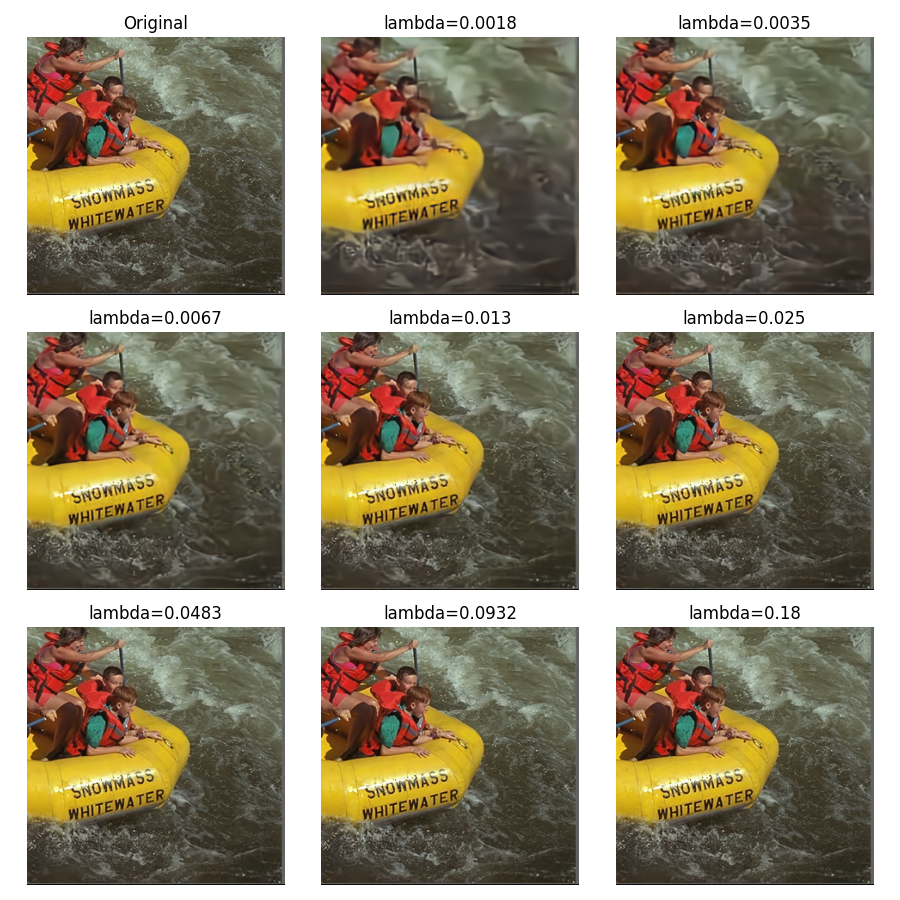
\includegraphics[width=15cm]{../img/bdpsnr_kodak_14_pretrained.png}
  \caption[Reconstruction results on image 14 of the Kodak dataset for different RD tradeoffs (pre-trained models).]{Reconstruction results on image 14 of the Kodak dataset for different RD tradeoffs (pre-trained models).}
  \label{appendix:bdpsnr_1:a}
\end{figure}

\begin{figure}
  \centering
  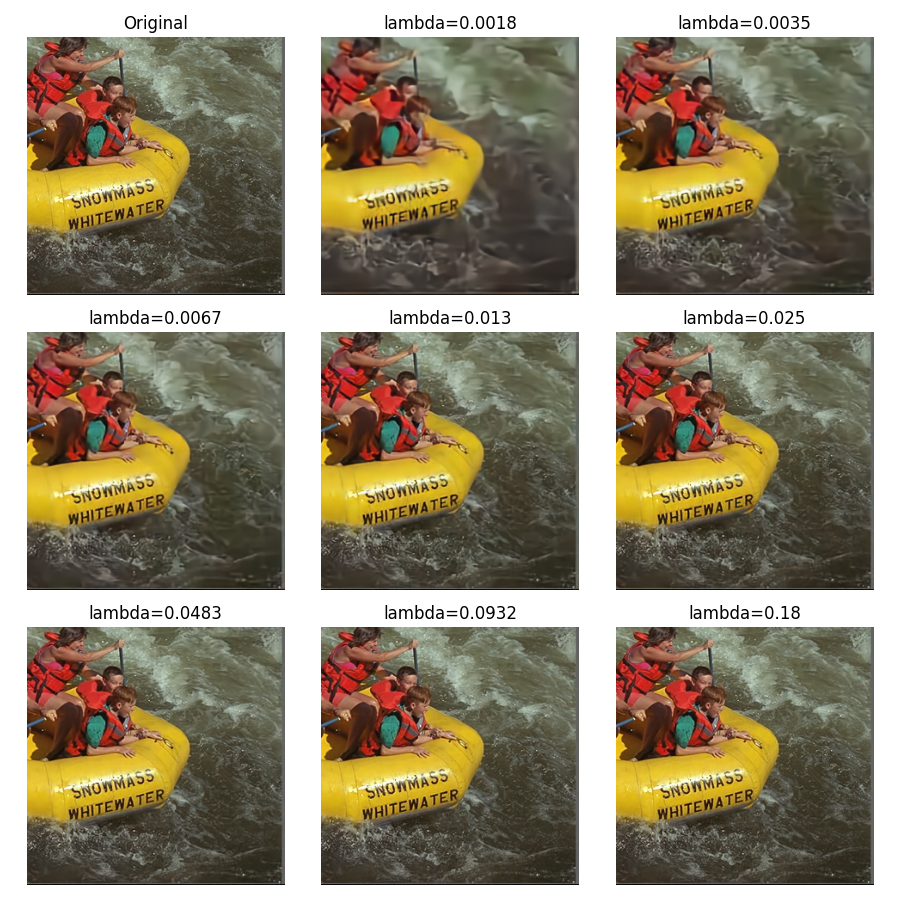
\includegraphics[width=15cm]{../img/bdpsnr_kodak_14.png}
  \caption[Reconstruction results on image 14 of the Kodak dataset for different RD tradeoffs (our models).]{Reconstruction results on image 14 of the Kodak dataset for different RD tradeoffs (our models).}
  \label{appendix:bdpsnr_1:b}
\end{figure}

\begin{figure}
  \centering
  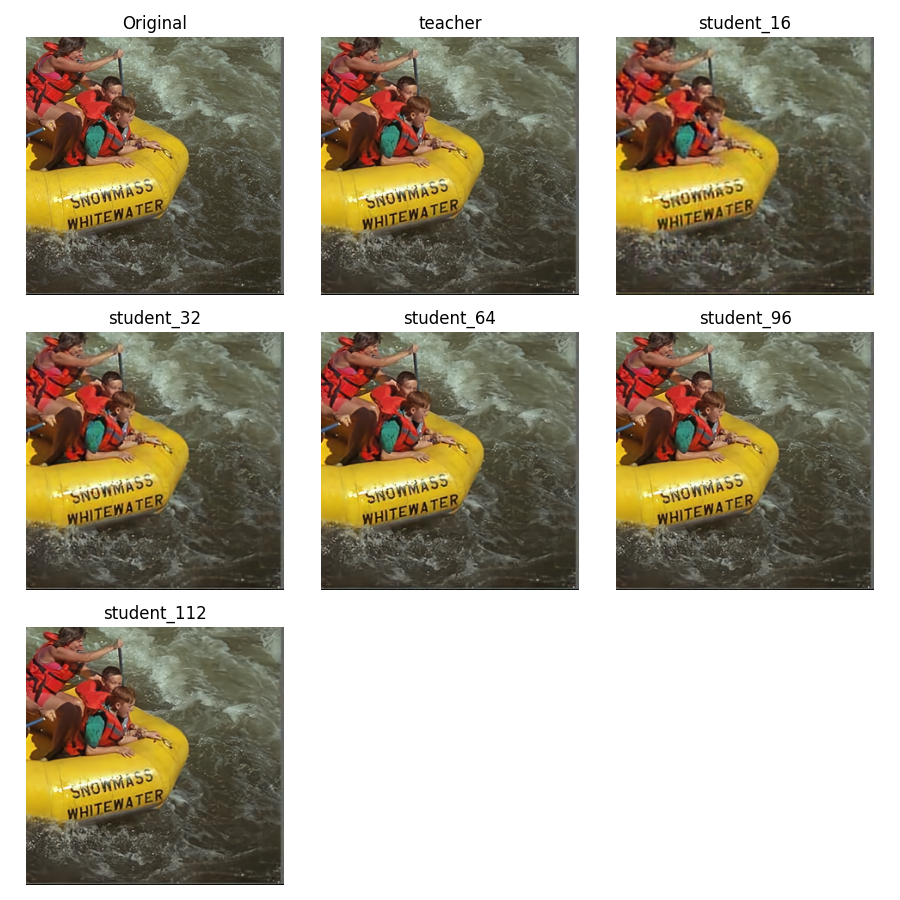
\includegraphics[width=15cm]{../img/kd_ae_kodak_14.png}
  \caption[Reconstruction results on image 14 of the Kodak dataset for image reconstruction with different architectures.]{Reconstruction results on image 14 of the Kodak dataset for image reconstruction with different architectures (pre-trained teacher with \textsf{quality} set to 5 and our student models with different number of channels trained for image reconstruction).}
  \label{appendix:kd_ae_1:a}
\end{figure}

\begin{figure}
  \centering
  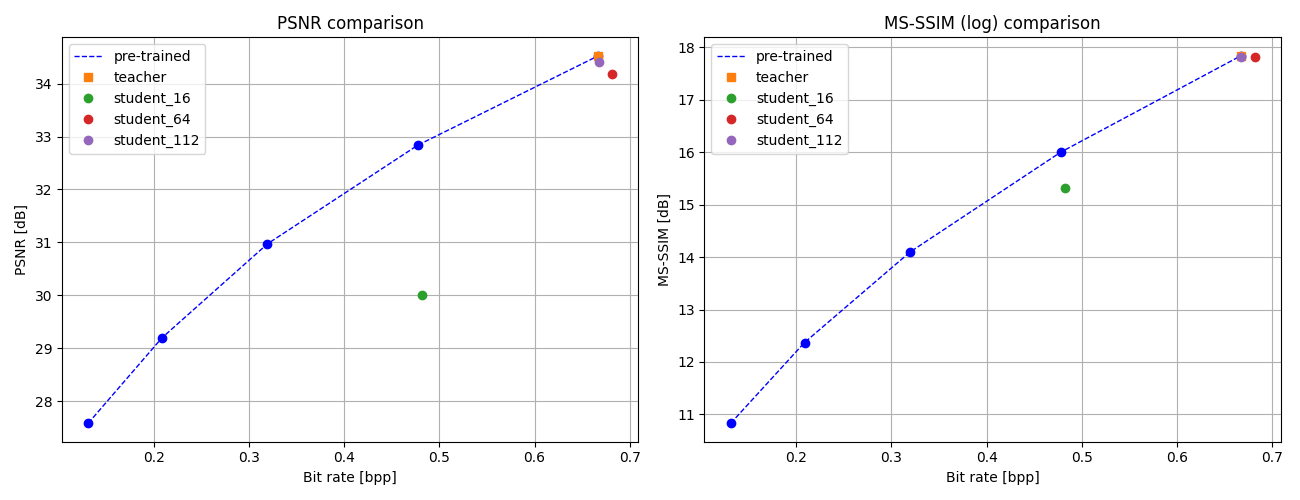
\includegraphics[width=15cm]{../img/kd_lic_rd_channels_kld.png}
  \caption[Average \acrshort{rd} curve on the Kodak dataset for students with different number of channels and Kullback-Leibler divergence loss on the latent space.]{Average \acrshort{rd} curve on the Kodak dataset for students with different number of channels and Kullback-Leibler divergence loss on the latent space.}
  \label{appendix:kd_lic_1_kld}
\end{figure}

\begin{figure}
  \centering
  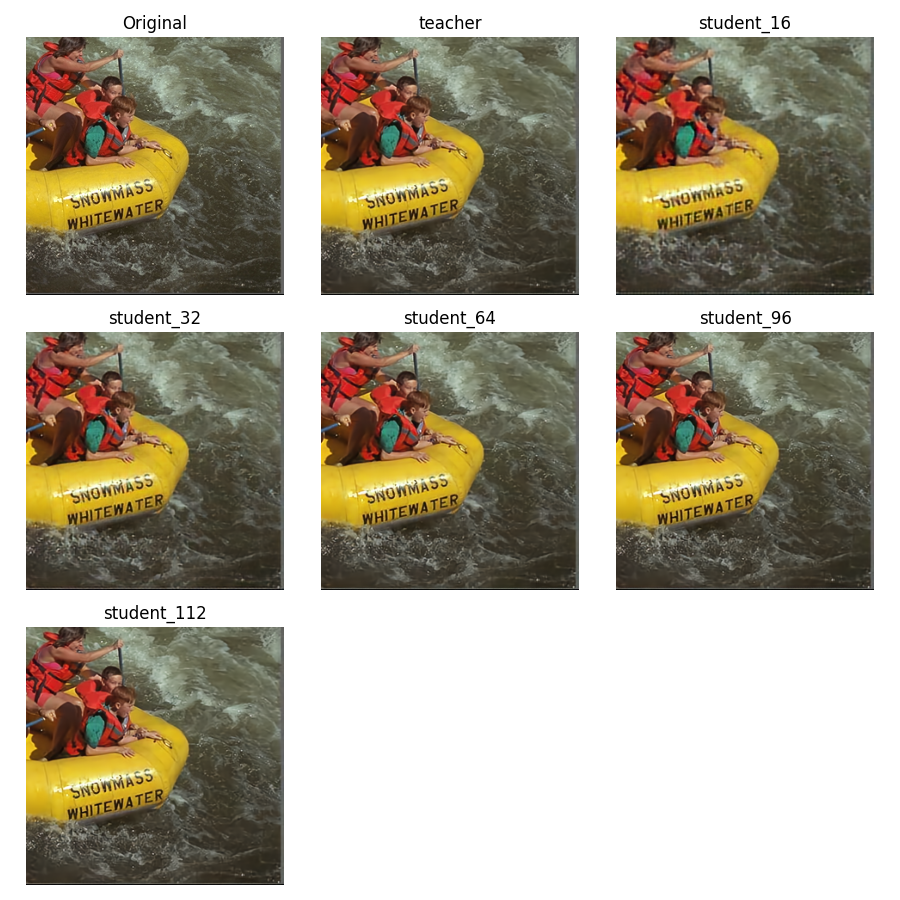
\includegraphics[width=15cm]{../img/kd_lic_kodak_14.png}
  \caption[Reconstruction results on image 14 of the Kodak dataset for image compression with different architectures.]{Reconstruction results on image 14 of the Kodak dataset for image compression with different architectures (pre-trained teacher with \textsf{quality} set to 5 and our student models with different number of channels trained for image compression).}
  \label{appendix:kd_lic_2:a}
\end{figure}

\begin{figure}
  \centering
  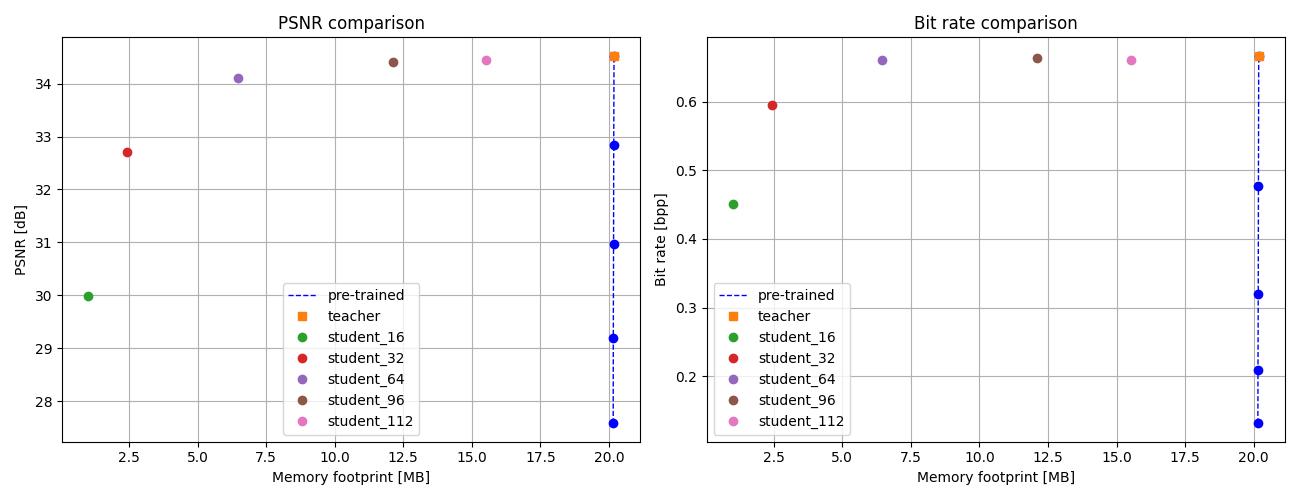
\includegraphics[width=15cm]{../img/kd_lic_memory.png}
  \caption[\acrshort{psnr} and bit rate on the Kodak dataset according to students memory footprint.]{\acrshort{psnr} and bit rate on the Kodak dataset according to students memory footprint.}
  \label{appendix:kd_lic_memory}
\end{figure}

\begin{figure}
  \centering
  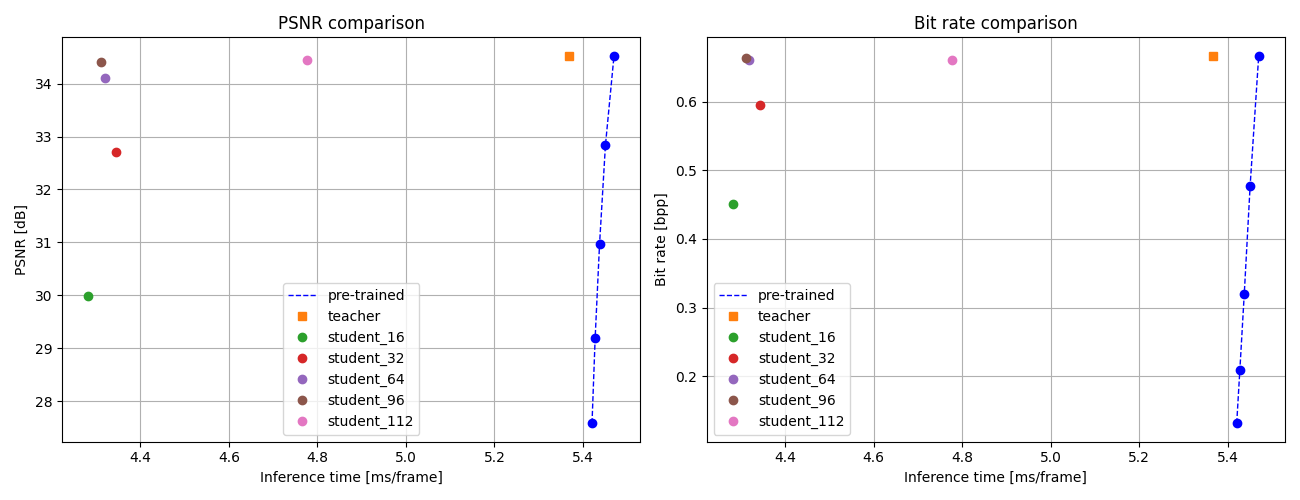
\includegraphics[width=15cm]{../img/kd_lic_time.png}
  \caption[\acrshort{psnr} and bit rate on the Kodak dataset according to students inference time.]{\acrshort{psnr} and bit rate on the Kodak dataset according to students inference time.}
  \label{appendix:kd_lic_time}
\end{figure}

\begin{sidewaystable}[]
  \centering
  \begin{tabular}{|c|c|lr|lr|lr|lr|lr|lr|lr|}
      \hline
      Model                     & \begin{tabular}[c]{@{}c@{}}Number\\ of channels\end{tabular} & \multicolumn{2}{c|}{\begin{tabular}[c]{@{}c@{}}Number of\\ parameters {[}M{]}\end{tabular}} & \multicolumn{2}{c|}{\begin{tabular}[c]{@{}c@{}}Memory\\ footprint {[}MB{]}\end{tabular}} & \multicolumn{2}{c|}{\begin{tabular}[c]{@{}c@{}}Floating point\\ operations\\ {[}GFLOP/frame{]}\end{tabular}} & \multicolumn{2}{c|}{\begin{tabular}[c]{@{}c@{}}Throughput\\ {[}FPS{]}\end{tabular}} & \multicolumn{2}{c|}{\begin{tabular}[c]{@{}c@{}}Energy\\ {[}mJ/frame{]}\end{tabular}} & \multicolumn{2}{c|}{PSNR}               & \multicolumn{2}{c|}{\begin{tabular}[c]{@{}c@{}}Bit rate\\ {[}bpp{]}\end{tabular}}      \\ \hline
      Teacher                   & 128                        & {\color[HTML]{656565} }                                  & 5.08                         & {\color[HTML]{656565} }                                  & 20.18                        & {\color[HTML]{656565} }                                  & 34.24                        & {\color[HTML]{656565} }                                  & 184.20                         & {\color[HTML]{656565} }                                  & 1767.85                         & {\color[HTML]{656565} }                                 & 34.53                         & {\color[HTML]{656565} }                                 & 0.67                         \\ \hline
                                & 112                        & {\color[HTML]{656565} -19.77 \%}                         & 4.07                         & {\color[HTML]{656565} -23.03 \%}                         & 15.53                        & {\color[HTML]{656565} -22.01 \%}                         & 26.70                        & {\color[HTML]{656565} +13.47 \%}                         & 209.01                         & {\color[HTML]{656565} -9.47 \%}                          & 1600.41                         & {\color[HTML]{656565} -0.26 \%}                         & 34.44                         & {\color[HTML]{656565} -1.03 \%}                         & 0.66                         \\ \cline{2-16} 
                                & 96                         & {\color[HTML]{656565} -37.47 \%}                         & 3.17                         & {\color[HTML]{656565} -40.01 \%}                         & 12.11                        & {\color[HTML]{656565} -41.31 \%}                         & 20.10                        & {\color[HTML]{656565} +25.74 \%}                         & 231.61                         & {\color[HTML]{656565} -19.88 \%}                         & 1416.34                         & {\color[HTML]{656565} -0.33 \%}                         & 34.41                         & {\color[HTML]{656565} -0.58 \%}                         & 0.66                         \\ \cline{2-16} 
                                & \cellcolor[HTML]{EFEFEF}64 & \cellcolor[HTML]{EFEFEF}{\color[HTML]{656565} -66.62 \%} & \cellcolor[HTML]{EFEFEF}1.69 & \cellcolor[HTML]{EFEFEF}{\color[HTML]{656565} -67.98 \%} & \cellcolor[HTML]{EFEFEF}6.46 & \cellcolor[HTML]{EFEFEF}{\color[HTML]{656565} -71.75 \%} & \cellcolor[HTML]{EFEFEF}9.67 & \cellcolor[HTML]{EFEFEF}{\color[HTML]{656565} +26.20 \%} & \cellcolor[HTML]{EFEFEF}232.47 & \cellcolor[HTML]{EFEFEF}{\color[HTML]{656565} -34.15 \%} & \cellcolor[HTML]{EFEFEF}1164.17 & \cellcolor[HTML]{EFEFEF}{\color[HTML]{656565} -1.21 \%} & \cellcolor[HTML]{EFEFEF}34.11 & \cellcolor[HTML]{EFEFEF}{\color[HTML]{656565} -0.91 \%} & \cellcolor[HTML]{EFEFEF}0.66 \\ \cline{2-16} 
                                & 32                         & {\color[HTML]{656565} -87.46 \%}                         & 0.64                         & {\color[HTML]{656565} -87.97 \%}                         & 2.43                         & {\color[HTML]{656565} -91.31 \%}                         & 2.98                         & {\color[HTML]{656565} +25.89 \%}                         & 231.90                         & {\color[HTML]{656565} -60.45 \%}                         & 699.18                          & {\color[HTML]{656565} -5.25 \%}                         & 32.71                         & {\color[HTML]{656565} -10.73 \%}                        & 0.60                         \\ \cline{2-16} 
      \multirow{-5}{*}{Student} & 16                         & {\color[HTML]{656565} -94.77 \%}                         & 0.27                         & {\color[HTML]{656565} -94.98 \%}                         & 1.01                         & {\color[HTML]{656565} -97.01 \%}                         & 1.02                         & {\color[HTML]{656565} +26.83 \%}                         & 233.63                         & {\color[HTML]{656565} -61.28 \%}                         & 684.45                          & {\color[HTML]{656565} -13.17 \%}                        & 29.98                         & {\color[HTML]{656565} -32.44 \%}                        & 0.45                         \\ \hline
  \end{tabular}
  \caption[Number of parameters, memory footprint, \acrshort{flop}s, throughput, consumed energy, \acrshort{psnr} and bit rate for teacher and student models.]{Number of parameters, memory footprint, \acrshort{flop}s, throughput, consumed energy, \acrshort{psnr} and bit rate for teacher and student models.}
  \label{appendix:tab_resources}
\end{sidewaystable}

\begin{figure}
  \centering
  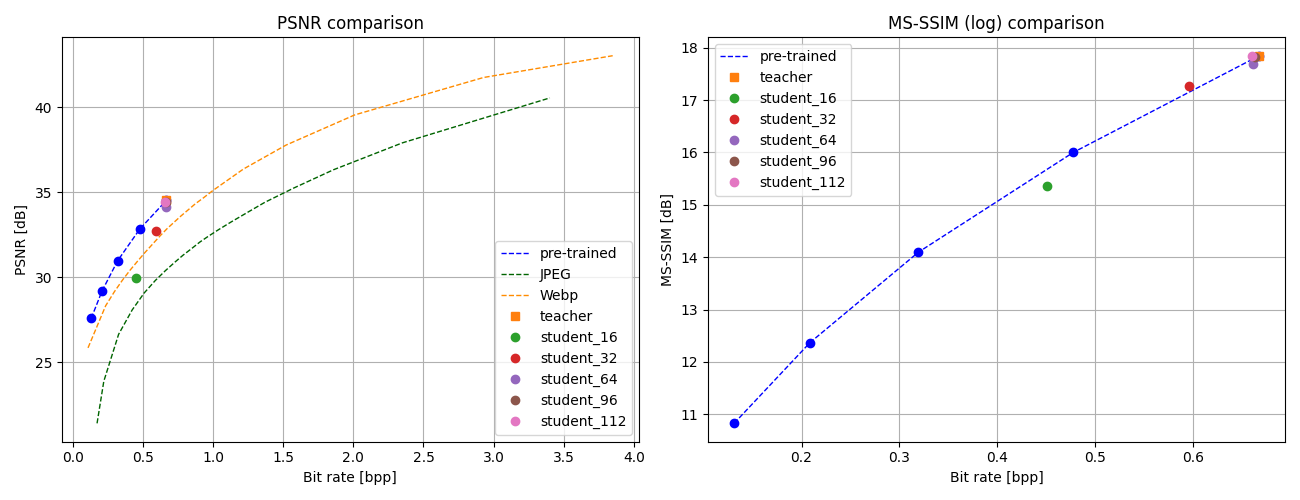
\includegraphics[width=15cm]{../img/codecs_rd.png}
  \caption[Average \acrshort{rd} curve on the Kodak dataset for students with different number of channels and codecs.]{Average \acrshort{rd} curve on the Kodak dataset for students with different number of channels and codecs.}
  \label{appendix:codecs_rd}
\end{figure}

\begin{figure}
  \centering
  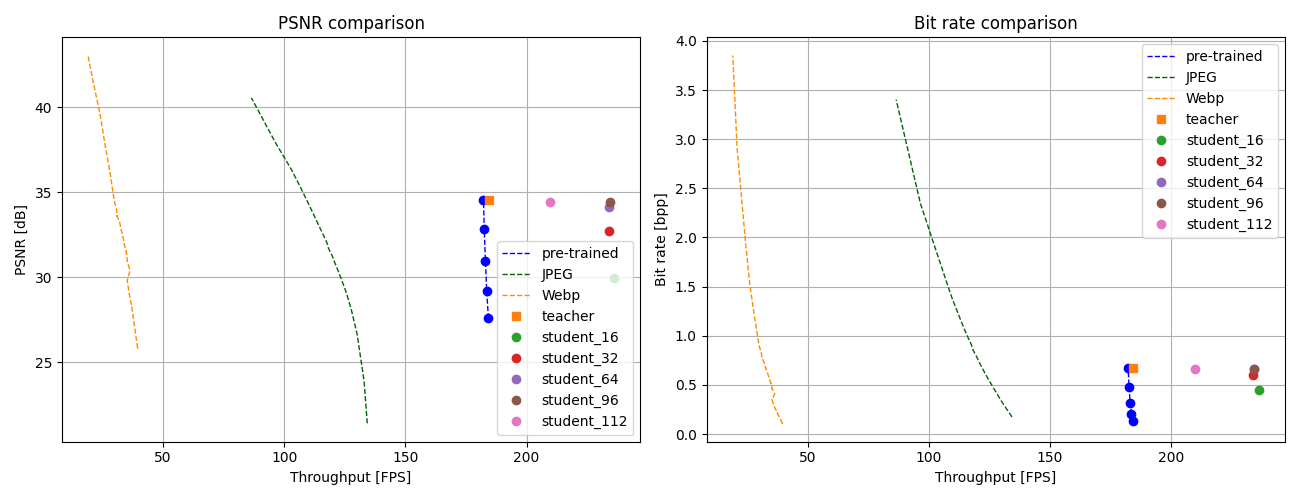
\includegraphics[width=15cm]{../img/codecs_fps.png}
  \caption[\acrshort{psnr} and bit rate on the Kodak dataset according to students and codecs throughput.]{\acrshort{psnr} and bit rate on the Kodak dataset according to students and codecs throughput.}
  \label{appendix:codecs_fps}
\end{figure}

\begin{figure}
  \centering
  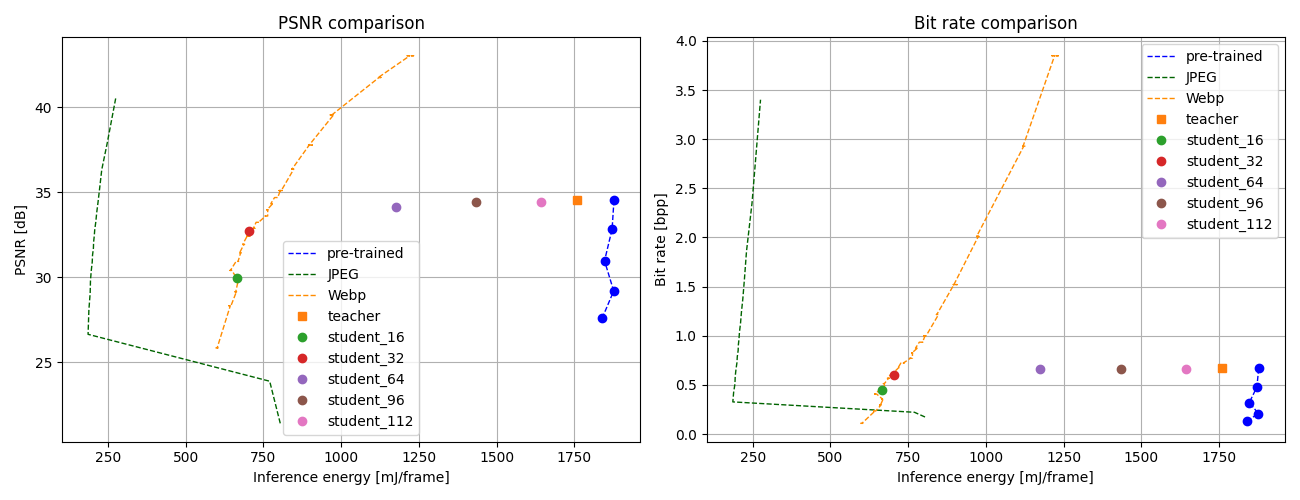
\includegraphics[width=15cm]{../img/codecs_energy.png}
  \caption[\acrshort{psnr} and bit rate on the Kodak dataset according to students and codecs consumed energy.]{\acrshort{psnr} and bit rate on the Kodak dataset according to students and codecs consumed energy.}
  \label{appendix:codecs_energy}
\end{figure}

\end{document}
